%%%%%%%%%%%%%%%%%%%%%%%%%%%%%%%%%%%%%%%%%%%%%%%%%%%%%%%%%%%%%%%%%%%%%%%%%%%%%%%%

\documentclass[12pt, a4paper, oneside]{book}

\input{/home/giatro/.config/user/giatro_packages.tex}

\input{/home/giatro/.config/user/giatro_macros.tex}

\title{Deep Learning\\\small{by DeepLearning.AI}}
\date{\today}
\author{Lucas Paiolla Forastiere}

%%%%%%%%%%%%%%%%%%%%%%%%%%%%%%%%%%%%%%%%%%%%%%%%%%%%%%%%%%%%%%%%%%%%%%%%%%%%%%%%
%%%%%%%%%%%%%%%%%%%%%%%%%%%%%%%%%%%%%%%%%%%%%%%%%%%%%%%%%%%%%%%%%%%%%%%%%%%%%%%%

\begin{document}

\maketitle
\tableofcontents
\newpage

%%%%%%%%%%%%%%%%%%%%%%%%%%%%%%%%%%%%%%%%%%%%%%%%%%%%%%%%%%%%%%%%%%%%%%%%%%%%%

\chapter{Introduction}%
\label{cha:introduction}

The term deep learning refers to training \textit{neural networks}, sometimes
very big neural networks. But what are neural networks?

So let's suppose we want to predict housing prices based on the size of the
house. And let's say we'll use Logistic Regression to do that. But as we know,
house prices can't be negative, so we simply say the value of the house is $0$
if the Logistic Regression would predict something negative.

That's indeed the simplest neural network we can have, we have a single input
\texttt{size} and a single output \texttt{price} and in the middle we have a
single neuron: the logistic regression.

\begin{figure}[h]
\centering
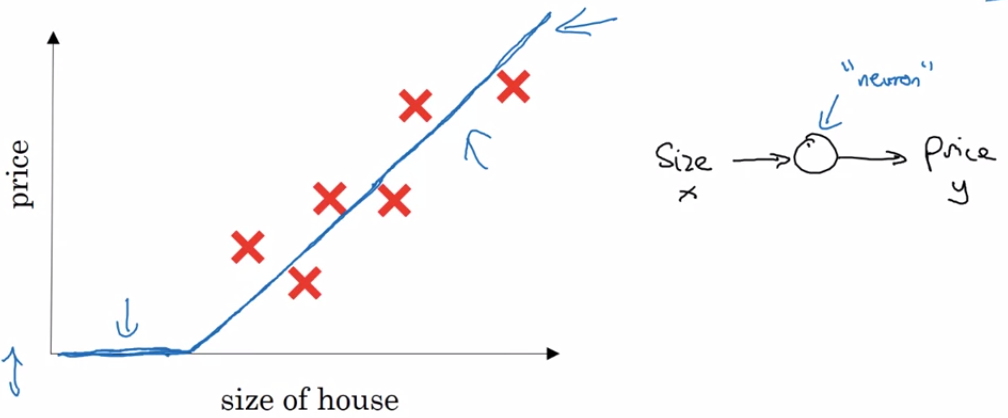
\includegraphics[scale=0.6]{Res/housing_logistic_regression.png}
\caption{Here we see the graph of the problem we described.}
\label{housing_logistic_regression.png}
\end{figure}

That function which is zero and than linear is called \textit{ReLU} and it's
used a lot in neural networks. It stands for \textit{Rectified Linear Unit}.

So to get a bigger neural network, we stack these neurons. Instead of predicting
using only the size of house, we could use the number of bedrooms, zip code and
wealth. We could use the size and number of bedrooms to predict the family size;
use the zip code to predict the walkability; and use the zip code and wealth to
predict the school quality. And then, we could use the family size, walkability
and school quality to predict the price. See in the picture:

\begin{figure}[h]
\centering
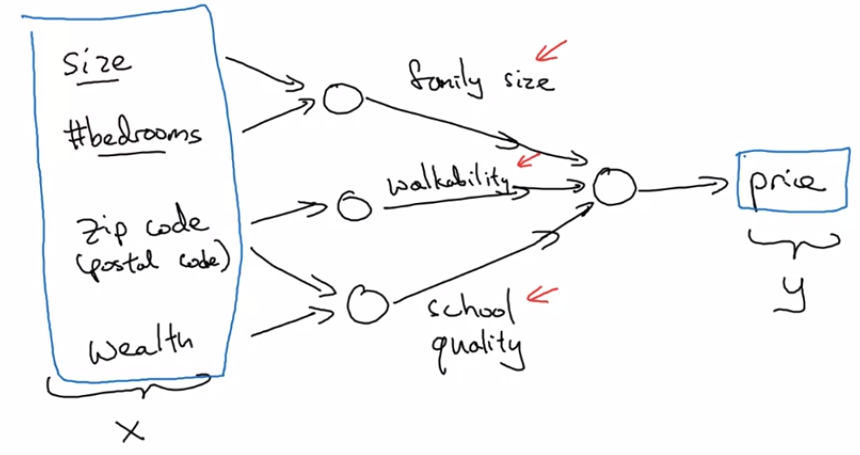
\includegraphics[scale=0.6]{Res/housing_nn.png}
\caption{Now we have a more complex neural network, which is the stack of many
ReLUs.}
\label{/housing_nn.png}
\end{figure}

However, in general what we have is something a little more complex than that.
We would have something like figure \ref{nn_generic.png}. Here we see that the
internal nodes (which are called \textbf{hidden nodes} or \textbf{hidden
neurons} or \textbf{hidden units}) receive the output of all the previous nodes
to make it predictions. These hidden nodes don't really have a meaning like the
example we gave. We don't try to predict family size or walkability or whatever,
we simply let the neural network decide what that neuron will output in order to
predict the final output \texttt{price} in the better way it can.

\begin{figure}[h]
\centering
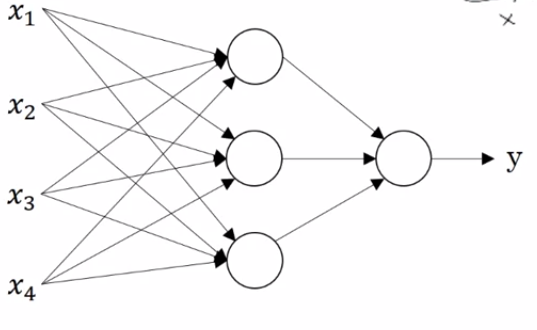
\includegraphics[scale=0.8]{Res/nn_generic.png}
\caption{The generic form of a neural network.}
\label{nn_generic.png}
\end{figure}

We can use neural networks in many applications, here we're going to foucos in
\textbf{supervised learning}, which are problems that you have a set of
variables called input (represented by $x$) and an output ($y$) related to that
input. In order to solve these kind of problems, there are many kinds of neural
networks. The one we saw is the most common one, but there are others, like
convolutional nn or recurrent nn.

\begin{figure}[h]
\centering
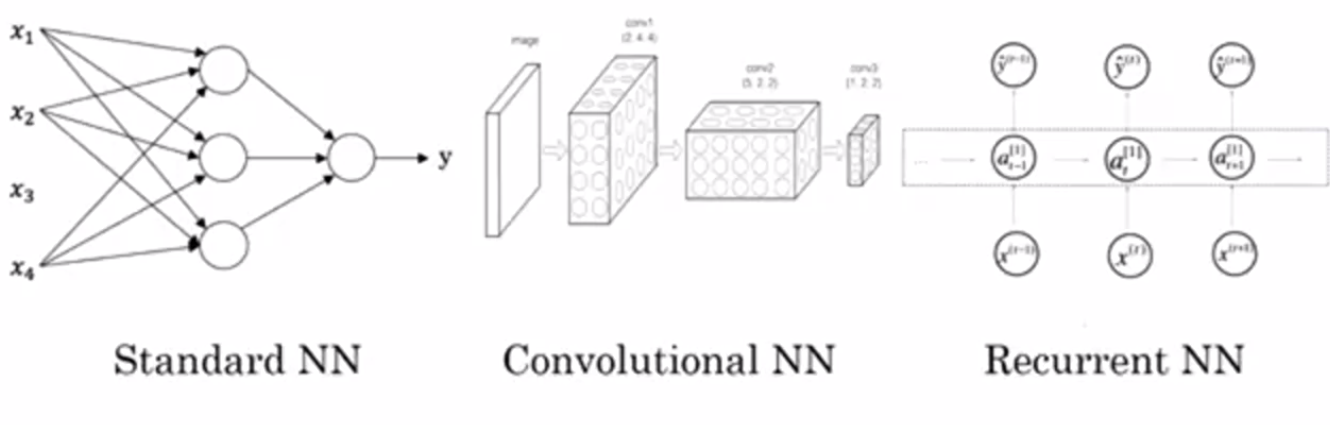
\includegraphics[scale=0.3]{Res/examples_nn.png}
\caption{Examples of neural networks.}
\label{examples_nn.png}
\end{figure}

Another thing that's important to decide what kind of nn we'll use is knowing if
the data we're leading with is \textit{structured} or \textit{unstructured}.

\textbf{Structured data} is data in the form of a table. We have a very clear
set of input variable $X$ and a set of output variables $y$. Each line of our
table represents one instance of data with many inputs and one or more outputs
related to those inputs.

\textbf{Unstructured data} is all the other kinds of data: audio, video, texts,
images, etc.

\begin{figure}[h]
\centering
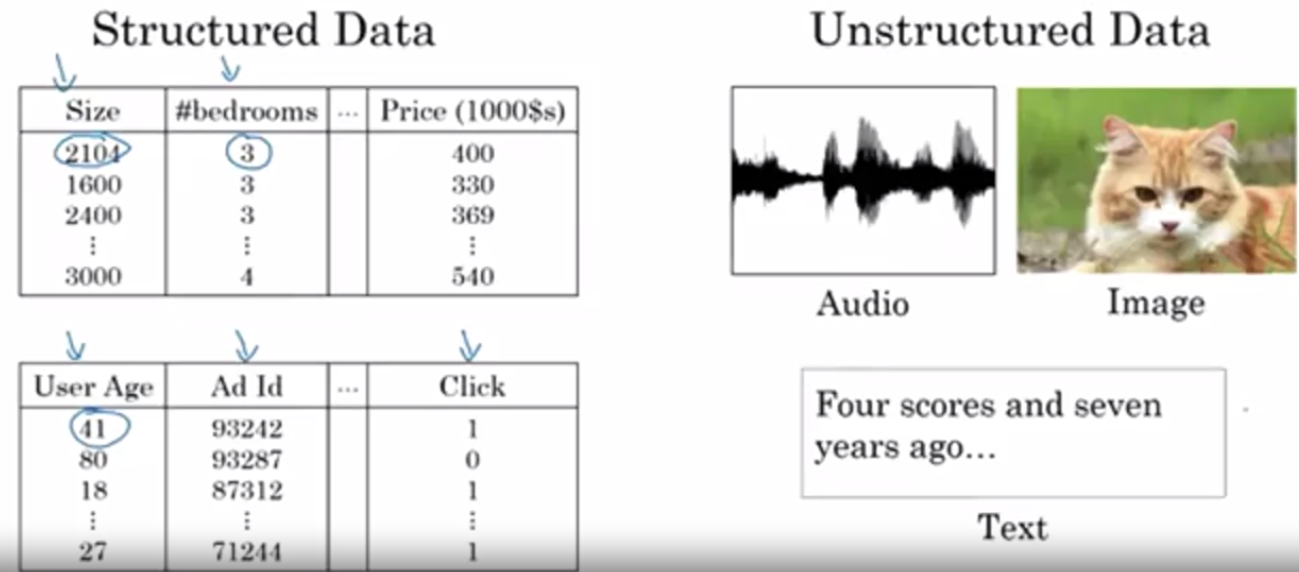
\includegraphics[scale=0.4]{Res/structured_vs_unstructed_data.png}
\caption{The two kinds of data.}
\label{structured_vs_unstructed_data.png}
\end{figure}

It turns out that machine learning algorithms performed better on structured
data over the years and more recently neural networks are performing better also
on unstructured data.

\paragraph{Why is Deep Learning taking off?}%
\label{par:why_is_deep_learning_taking_off_}

This is one of the questions we must ask ourselves when begining to learn deep
learning. Let's see the graph of the performance of the machine learning
algorithms versus the amount of data that we provide to then. We see that
traditional learning algorithms have a plato where they can't improve anymore,
which neural networks can lead with that data as we make than bigger and bigger.

\begin{figure}[h]
\centering
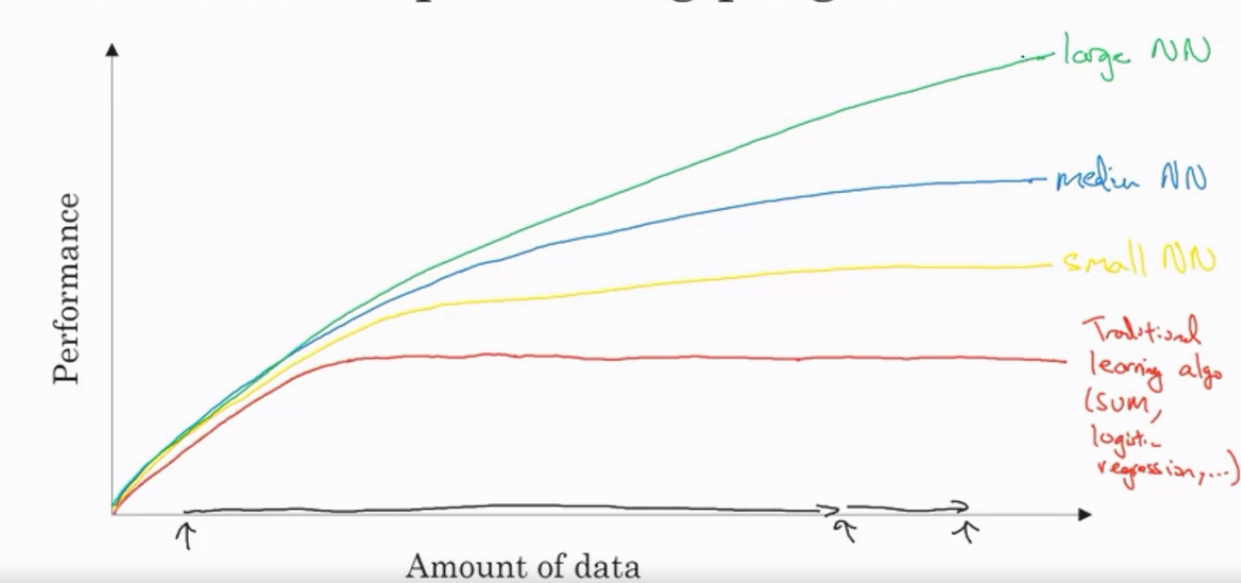
\includegraphics[scale=0.4]{Res/ml_algorithms_performance.png}
\caption{The performance of machine learning algorithms in respect to the data
we provide to them.}
\label{ml_algorithms_performance.png}
\end{figure}

We also see in the graph that when we don't have a large amount of data, NNs
all algorithms perform pretty much the same.

So in order to answer our question, we have to understand the evolution of three
things: \textit{data}, \textit{computation} and \textit{algorithms}.

Through the years, the amount of data available was inscreased a lot, so NNs can
take advantage from that. Also the computation power was inscreased with the use
of GPUs to make a large amount of computations. And finally new algorithms have
been developed to make NNs faster. That's the main reason why deep learning is
taking off.

\section{Notation}%
\label{sec:notation}

Before continuing, we need to define the notation we're going to use.

\begin{itemize}
    \item $(x,y)$ will denote a single training input;
    \item $m$ or $m_{\text{train}}$ denotes the number of training examples;
    \item $\xii[x]{i}$ denotes the $i$-th training input;
    \item $\xii[y]{i}$ denotes the $i$-th traning output;
    \item $n_x$ or $n$ denotes the number of dimensions $x$ has (or the number
        of features);
    \item $m_{\text{test}}$ denotes the number of testing examples;
    \item $X$ is the matrix of all traning examples. It's defined as:
        \[
        X = \begin{bmatrix}
            | & | &  & | \\
            \xii[x]{1} & \xii[x]{2} & \cdots & \xii[x]{m} \\
            | & | &  & | \\
        \end{bmatrix}
        \]
        $X$ is an $m\times n$ matrix;
    \item $Y$ is the matrix of all outputs. It's defined as:
        \[
        Y = \begin{bmatrix}
            \xii[y]{1} & \xii[y]{2} & \cdots & \xii[y]{m}
        \end{bmatrix}
        \]
        $Y$ is a $1\times m$ matrix.
\end{itemize}

\begin{obs}
In other courses we might see $X$ defined as the transpouse of the matrix we've
just defined. But it turns out that when using this definiting, it's much easier
to implement algorithms, so remember te definition we're going to use through out
the course.

The same thing for $Y$. We see that here $Y$ is the transpouse of that it's
tends to be in other courses.
\end{obs}

\section{Logistic Regression as a Neural Network}%
\label{par:logistic_regression_as_a_neural_network}

To end this introduction, we'll see the basics of neural network programming
using the simplest NN we can: a logistic regression.

So let's recall what's logistic regression and why it's useful. Logistic
Regression is used in binary classification, the kind of problem where we have
an input and want to predict between $0$ or $1$. An example could be an image
and we want to say it what's a cat ($1$) or not ($0$).

Basicly we want an algorhthm to estimate the probability of $y=1$ given $x$. In
math we write:
\[
    \hat{y}=P(y=1\cond x),\t\t x\in\R^{n}
\]

Logistic Regression estimates this quantity using the formula:

\[
    \hat{y}=\sigma(w^{T}x+b),
\]
where $w$ and $b$ are parameters to be discovered and $\sigma$ is the
\textbf{sigmoid function}:

\[
    \sigma(z) = \dfrac{1}{1+e^{-z}}
\]

\begin{figure}[h]
\centering
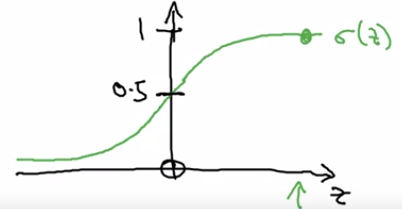
\includegraphics[scale=0.7]{Res/sigmoid.png}
\caption{A sigmoid graph.}
\label{sigmoid.png}
\end{figure}

It's also common to create a new input $x_0=1$ and use the $x$ vector as
$x\in\R^{n+1}$ and use the formula $\hat{y}=\sigma(\theta^{T}x)$, where

\[
\theta=\begin{bmatrix}
    \theta_0 \\ \theta_1 \\ \theta_2 \\ \vdots \\ \theta_n
\end{bmatrix}\t \theta_0=b\t w=\begin{bmatrix}
    \theta_1 \\ \theta_2 \\ \vdots \\ \theta_n
\end{bmatrix}
\]

To find the parameters $b$ and $w$, we need to define a \textbf{cost function},
which is a function that says how badly our algorithm is performing. This is a
function that we want to minimize and when we minimize, we find the best values
of $b$ and $w$.

The \textbf{cost} function is a function of all training examples, while a
\textbf{loss function} or \textbf{error function} is a function of a single
traning example that measures how well our algorithm is performing.

For logistic regression, we use the loss function:

\[
    \mathcal{L}(\hat{y},y)=-y \log\hat{y}-(1-y)\log(1-\hat{y})
\]

Notice that this is the same as:
\[
    \mathcal{L}(\hat{y},y)=\begin{cases}
        -\log(\hat{y}-1), &\text{ if } y=0\\
        -\log\hat{y}, &\text{ if } y=1\\
    \end{cases}
\]

That give us the cost function:
\[
    J(w,b)=\dfrac{1}{m}\spsum{i=1}{m}\mathcal{L}(\xii[\hat{y}]{i},\xii[y]{i})
\]

\subsection{Gradient Descent}%
\label{sub:gradient_descent}

We know have:
\begin{itemize}
    \item A way of predicting the classes $0$ or $1$ using the sigmoid function;
    \item A way of measuring the error of our predictions.
\end{itemize}

What we need now is a way of chaning our parameters $b$ and $w$ in order to
minimize the error. That's what the \textbf{gradient descent} algorithm does.

Let's first see a general graph of the cost function. In general, it looks like
figure \ref{Cost_function.png}

\begin{figure}[h]
\centering
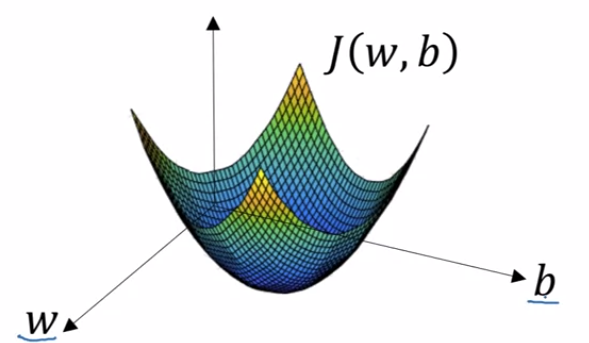
\includegraphics[scale=0.8]{Res/Cost_function.png}
\caption{A generic graph of the cost function.}
\label{Cost_function.png}
\end{figure}

We see that $J$ is what we call a \textbf{convex function}, which means that it
is a function that was only one \textbf{local minimum} (or local maxima). This
property is very important if we want to apply the gradient descent algorithm.

In Gradient Descent, we initialize $b$ and $w$ randomly and take steps into the
direction that leads us to the lowest possible value of $J$. In order to do
that, we calculate the \textbf{gradient} (the derivatives in each direction) of
the function $J$ and take a step in the opposite direction of the gradient.

\begin{prop}
The gradient gives us the direction of the maximum increase of the a function.
\end{prop}

\begin{algorithm}[Gradient Descent]
Repeat \{ \nl
\t $w:=w-\alpha\parderiv[w]{J(w,b)}$ \nl
\t $b:=b-\alpha\parderiv[b]{J(w,b)}$ \nl
\}
\end{algorithm}

In the algorithm, $\alpha$ is what we call the \textbf{learning rate}. It's how
large we should step in the direction of the maximum decrease. If we take big
steps, we can go much faster to the global minumum, but we might not be so
accurated. On the other hand, we be take small steps, we can find the global
minum accuratedly, but achieve it much slower.

Gradient Descent is a general optimization algorithm and can be applied to any
convex function. So now we need to understand how to use it with logistic
regression.

After calculating the derivatives, we'll have:

\begin{algorithm}[Gradient Descent for Logistic Regression]
Repeat \{ \nl
\t$J=0;~dw=0;~db=0$ \nl
\t For $i=1\cdots m$:\nl
\t\t $\xii[z]{i}=w^{T}\xii[x]{i}+b$\nl
\t\t $\xii[a]{i}=\sigma(\xii[z]{i})$\nl
\t\t $J+=
-\sbracket{\xii[y]{i}\log\xii[a]{i}+(1-\xii[y]{i})\log(1-\xii[a]{i})}$\nl
\t\t $d\xii[z]{i}=\xii[a]{i}-\xii[y]{i}$\nl
\t\t $dw += \xii[x]{i}d\xii[z]{i}$\nl
\t\t $db += d\xii[z]{i}$\nl
\t $J/=m$\nl
\t $dw/=m;~db/=m$\nl
\t $w:=w-\alpha dw$ \nl
\t $b:=b-\alpha db$ \nl
\}
\end{algorithm}

This version of the algorithm uses a for loop to compute $J$, $dw$ and $db$. But
when implementing the code into Python or other language, we always try to
\textbf{vectorize} the code to make it faster.

\begin{algorithm}[Gradient Descent for Logistic Regression Vectorized]
Repeat \{ \nl
\t $Z=w^{T}X+b$ \nl
\t $A=\sigma(Z)$ \nl
\t $dZ = A - Y$ \nl
\t $dw = \dfrac{1}{m}XdZ^{T}$ \nl
\t $db = \dfrac{1}{m}\spsum{}{}dZ$ \nl
\t $w:=w-\alpha dw$ \nl
\t $b:=b-\alpha db$ \nl
\}
\end{algorithm}

%%%%%%%%%%%%%%%%%%%%%%%%%%%%%%%%%%%%%%%%%%%%%%%%%%%%%%%%%%%%%%%%%%%%%%%%%%%%%

\chapter{Basical Concepts}%
\label{cha:basical_concepts}

So let's start introducing some notation.

Whenever we use:
\[
    \xlayer[z]{i}
\]

we're talking about the $z$ values of the $i$-th \textit{layer} of the neural
network.

Thus, we have the following important equation:


\begin{equation}
\boxed{
    \xlayer[z]{i} = \xlayer[W]{i}\xlayer[a]{i-1} + \xlayer[b]{i}}
\label{forward-z}
\end{equation}

\begin{equation}
\boxed{
    \xlayer[a]{i} = \sigma(\xlayer[z]{i})}
\label{foward-activation}
\end{equation}

\section{Representation}%
\label{sec:representation}

Let's ilustrate a simple neural net:

\begin{figure}[h]
\centering
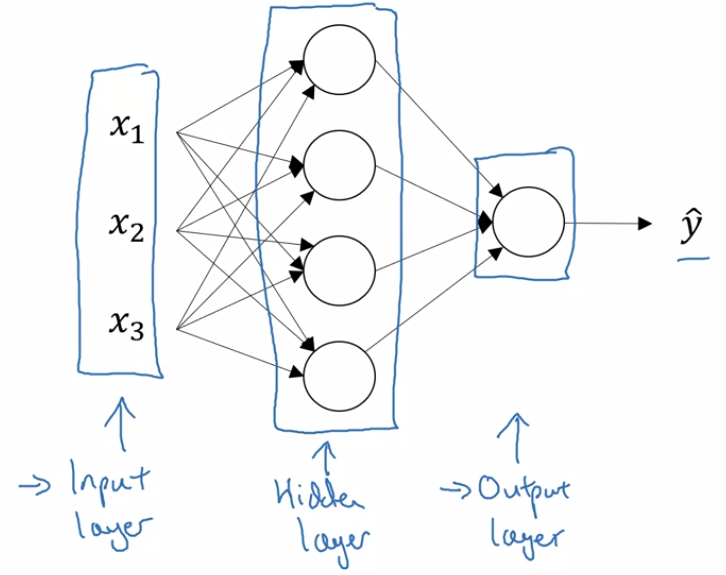
\includegraphics[scale=0.5]{Res/nn_representation.png}
\label{nn_representation.png}
\end{figure}

This nn is divided into three parts:
\begin{itemize}
    \item The \textbf{input layer} is the layer were we enter the data, the
        features.  It's represented by a single vector $x$, which is a column of
        our inputs matrix $X$. Another way to denote the input is by
        $\xlayer[a]{0}$;
    \item The \textbf{output layer} is the layer were we get our answer. It can
        be one of more nodes and it's represented by a single vector $y$. It can
        be a binary vector, continuous vector, it could be even a codification
        of an image, sound, word or any codification just like the input;
    \item Finally, the \textbf{hidden layer} are all the nodes which are between
        the input and output, they are the intermediately computations that our
        neural net does. We don't need to stick to just one hidden layer, there
        could be many of them.
\end{itemize}

One more thing to keep in mind is that the neural network drawn in the picture
is called a \textit{two layer} neural network, because we don't count the input
layer as a ``real'' layer (it's the layer zero).

Each layer (real layer) will have \textbf{parameters} associated with them,
which we'll denote $\xlayer[W]{i}$ and $\xlayer[b]{i}$ for the $i$-th layer.

To understand what are node computes given an input, let's focus in the first
node of the hidden layer in the figure. We can see that the inputs $x_1,x_2,x_3$
are all passed to that node, which uses tham to output something to the node in
the output layer (or it could be outputed to the next hidden layer).

So basicaly a node is a logistic regression, it computes:
\[
    a = \sigma(Wx+b)
\]

But as we have many computations like this, we have to use indeces to denote the
first hidden layer and the first node of that layer. So the computations would
be described as following:

\[
\xlayer[z]{1}_1=\xlayer[W]{1}_1^{T}x+\xlayer[b]{1}_1
\]
\[
\xlayer[a]{1}_1=\sigma(\xlayer[z]{1}_1)
\]

The superscript means we're talking about the first (real) layer and the
subscript means we're talking about the first node of that layer. Therefore
$\xlayer[a]{l}_i$ is the \textbf{activation value} (output value) of the $i$-th
node in the $l$-th layer.

Of course, when coding a neural network, we don't compute each one of these
equations using a for loop, we vectorize in order to compute the whole vector
$\xlayer[z]{l}$ at once using equation \ref{forward-z}.

\paragraph{Vectorizing the input}%
\label{par:vectorizing_the_input}

Now, one more thing that we want is to be able to predict \textit{mulpible}
inputs at once. Indeed we can do that with some vectorization. Let's see how.

So let's recall that
\[
X = \begin{bmatrix}
    | & | &  & | \\
    \xii[x]{1} & \xii[x]{2} & \cdots & \xii[x]{m} \\
    | & | &  & | \\
    \end{bmatrix}
\]
and let's define a matrix $\xlayer[Z]{l}$ in which the $j$-th column is the
vector $z^{[l](j)}$ (i.e., the value before the activation function of the layer
$l$ when applied to the input $j$).

\[
\xlayer[Z]{l} = \begin{bmatrix}
    | & | &  & | \\
    z^{[l](1)} & z^{[l](2)} & \cdots & z^{[l](m)} \\
    | & | &  & | \\
    \end{bmatrix}
\]

and also define the matrix $\xlayer[A]{l}$, which is $\sigma(\xlayer[Z]{l})$:

\[
\xlayer[A]{l} = \begin{bmatrix}
    | & | &  & | \\
    a^{[l](1)} & a^{[l](2)} & \cdots & a^{[l](m)} \\
    | & | &  & | \\
    \end{bmatrix}
\]

We can see that each row of matrix $A$ tell us the activation value for a
particular node of that layer for each input. For instance, the value
$A^{[l]}_{i,j}$ is the value of the $i$-th neuron in the $l$-th layer of the
neural network when we input the $j$-th input.

Given these matrices, we can train over all inputs using the vectorized formula:

\begin{equation}
    \boxed{\xlayer[Z]{l}=\xlayer[W]{l}\xlayer[A]{l-1}+\xlayer[b]{l}}
\end{equation}

\begin{equation}
    \boxed{\xlayer[A]{l}=\sigma(\xlayer[Z]{l})}
\end{equation}

and recall that $X=\xlayer[A]{0}$.

\section{Activation Functions}%
\label{sec:activation_functions}

The \textbf{activation function} is the function $g$ applied to $z$. We've
been currently using the \textit{sigmoid function} $\sigma$, but there are some
other functions that can be used and can significatly change our results and
performances.

Another function one can use is the $\tanh$ function, given by the formula:
\[
    \tanh(z) = \dfrac{e^{z}-e^{-z}}{e^{z}+e^{-z}}
\]

which is a shifted version of the sigmoid function. We have $\tanh(0)=0$ instead
of $\sigma(0)=0.5$.

It turns out that the $\tanh$ function frequently works better than the sigmoid,
because the values are between $-1$ and $1$ instead of $0$ and $1$ and thus the
average values tend to be closer to zero.

The exception is for the output layer, where it's good to have a number between
$0$ and $1$ in many cases, so we could keep using the sigmoid function there and
use the tanh on the hidden layers.

One of the down sides of these two functions is that when $z$ is very large, the
gradient is very small, because they're very flat for large (positive or
negative) values of $z$.

That's why many times we see the \textbf{ReLU} (rectified linear unit) function
being used:

\[
    ReLU(z) = \dmax(0,z)
\]

Indeed the ReLU is the most used activation in practice and should be the first
choise. One of the only down sides of it is that the derivative for values lower
than zero is zero, but it works fine in practice.

There's modified version of the ReLU called \textbf{Leaky ReLU}, which is given
by:

\[
    LReLU(z) = \dmax(0.01z,z)
\]

It's just like the ReLU function, but it's not zero for any negative value of
$z$ and, thus, the derivative is not null on those points. Actually, indeed
there no reason for the $0.01$, it could be any small value and we can turn that
into a hyperparameter of our algorithm.

\paragraph{Why activation functions}%
\label{par:why_activation_functions}

Now that we've seen so many activation functions we might want to understand why
do we even need them. And most importantly, why do we need they to be
non-linear.

We could try using $a=g(z)=z$ (i.e., doing nothing). It turns out that if we
have just the identity function, we can't express \textit{complex} (non-linear)
decision boundaries.

We'll not prove it here, but if we just use a linear function in all hidden
nodes and a sigmoid, it is equivalent to a standard logistic regression in terns
of what it can express.

\begin{align*}
\xlayer[a]{1}&=\xlayer[w]{1}x+\xlayer[b]{1} \\ \\
\xlayer[a]{2}&=\xlayer[w]{2}\xlayer[a]{1}+\xlayer[b]{2} \\
             &=\xlayer[w]{2}\paren{\xlayer[a]{1}=\xlayer[w]{1}x+\xlayer[b]{1}}+
             \xlayer[b]{2} \\
             &=\paren{\xlayer[w]{2}\xlayer[w]{1}}x+
             \paren{\xlayer[w]{2}\xlayer[b]{1}+\xlayer[b]{2}}=\\
             &=w'x+b'
\end{align*}

Above we can see that from one layer to the next we still have a linear
equation (a composition of two linear functions is a linear function).

\section{Backpropagation}%
\label{sec:backpropagation}

Now we're going to understand how to find the optimal values for $W$ and $b$
using backpropagation.

The first step in this direction is calculating the derivative of the activation
functions. So let's to it.

\paragraph{Sigmoid}%
\label{par:sigmoid}

\[
    g(z)=\dfrac{1}{1+e^{-z}}
\]
\begin{align*}
    \deriv[z]{g(z)}&=\dfrac{1}{1+e^{-z}}\paren{1-\dfrac{1}{1+e^{-z}}} \\
                   &= g(z)(1-g(z))
\end{align*}

\paragraph{Tanh}%
\label{par:tanh}

\[
    g(z)=\tanh(z)
\]
\begin{align*}
    \deriv[z]{g(z)}&=1-\paren{\tanh(z)}^2 \\
                   &=1-g(z)^2
\end{align*}

\paragraph{ReLU}%
\label{par:relu}

\[
    g(z)=\dmax(0,z)
\]
\[
    \deriv[z]{g(z)}=\begin{cases}
        0, &\text{ if }z<0 \\
        1, &\text{ if }z>0 \\
        \text{undef}, &\text{ if }z=0
    \end{cases}
\]

\paragraph{Leaky ReLU}%
\label{par:leaky_relu}

\[
    g(z)=\dmax(0.01z,z)
\]
\[
    \deriv[z]{g(z)}=\begin{cases}
        0.01, &\text{ if }z<0 \\
        1, &\text{ if }z>0 \\
        \text{undef}, &\text{ if }z=0
    \end{cases}
\]

Now let's understand how to do \textbf{gradient descent}.

Let's denote $L$ the number of layers of our network. Them, the last value
derivative (the first we're going to compute) is given by the formula:

\begin{equation}
    \xlayer[dz]{L}=\xlayer[a]{L}-y
    \label{last-dz}
\end{equation}

The values of $dW$ and $db$, for any layer are given by the formulas:

\begin{align}
    \xlayer[dW]{l}&=\xlayer[dz]{l}\xlayer[a]{l-1}^{T} \\
    \xlayer[db]{l}&=\xlayer[dz]{l}
    \label{dW-db}
\end{align}

The other values of $dz$ for any layer other than the output layer are given by
the formulas:

\begin{equation}
    \xlayer[dz]{l}=\xlayer[W]{l+1}^{T}\xlayer[dz]{l+1}*
    \xlayer[g]{l}'\paren{\xlayer[z]{l}}
    \label{dz-equation}
\end{equation}

where $*$ denotes que \textit{element-wise} product.

There's also a vectorized way of computing this for all the training examples at
once.

\begin{align}
    \xlayer[dZ]{L}&=\xlayer[A]{L}-Y \\
    \xlayer[dW]{l}&=\dfrac{1}{m}\xlayer[dZ]{l}\xlayer[A]{l-1}^{T} \\
    \xlayer[db]{l}&=\dfrac{1}{m}\text{sum}\paren{\xlayer[dZ]{l}, \text{axis=1})}
        \\
    \xlayer[dZ]{l}&=\xlayer[W]{l+1}^{T}\xlayer[dZ]{l+1}*
    \xlayer[g]{l}'\paren{\xlayer[Z]{l}}
\end{align}

\section{Random Initialization}%
\label{sec:random_initialization}

Finanlly, we need to initialize the parameters of the neural network. It turns
out that initializing everything as zero or everything as the same number, then
all nodes of a layer will be exactly the same even with many iterations of
gradient descent.

For the values of $b$, we can initialize with zero, but for $W$, we prefer to
initialize with \textit{small} random numbers. We like the numbers to be small
though because if we're using $\tanh$ or $\sigma$, big numbers will have a very
plat derivative and, thus, the algorithm will learn slower.

\section{Notation for deep neural networks}%
\label{sec:notation_for_deep_neural_networks}

We'll use $L$ to describe the number of layers the neural network have
(remember, the input layer is not a real layer).

$\xlayer[n]{l}$ denotes the number of nodes on layer $l$.

$\xlayer[a]{l}$ denotes the activation values on layer $l$.

$\xlayer[g]{l}$ denotes the activation function used on layer $l$.

Also, the dimensions of $\xlayer[W]{l}$ and $\xlayer[b]{l}$ are
$\pair{\xlayer[n]{l}}{\xlayer[n]{l-1}}$ and $\pair{\xlayer[n]{l}}{1}$.

%%%%%%%%%%%%%%%%%%%%%%%%%%%%%%%%%%%%%%%%%%%%%%%%%%%%%%%%%%%%%%%%%%%%%%%%%%%%%%%%

\chapter{Practical Aspects of Deep Learning}%
\label{cha:practical_aspects_of_deep_learning}

In this chapter we're going to focus on the practical aspects of deep learning,
like how to choose the hyperparameters, how to make the code faster, how to
apply regularization and others.

The first thing to understand is that, in practical, we divide our data set
into three:
\begin{itemize}
    \item \textit{Training set}, in which we're going to train the model;
    \item \textit{Hold-out cross validation set (or dev set)}, in which we're
        going to evaluate our model and choose hyperparameters;
    \item \textit{Test set}, in which we're going to evaluate our final model,
        with the hyperparameters setted.
\end{itemize}

In the previous era of Machine Learning, we would use $70\%$ for the
training/dev sets and $30\%$ for testing, or $60/20/20\%$. But now in the big
data era, we can use much small fractions for the testing and hold-out sets
(like $1\%$ or even less, since this can be equivalent to about $10000$
examples).

Another important thing to keep in mind is that the training set and test set
must have the \textit{same distribution} of that. For instance, if we train on
images of cats coming from the web, than we should not test on images of cats
coming from mobile cameras.

\section{Regularization}%
\label{sec:regularization}

We've seen that the cost function of our neural network is a function $J$ such
that:

\[
    J\paren{\xlayer[W]{1},\xlayer[b]{1},\cdots,\xlayer[W]{L},\xlayer[b]{L}}=
    \dfrac{1}{m}\spsum{i=1}{m}\mathcal{L}(\hat{\xii[y]{i}},\xii[y]{i})
\]

\textbf{Regularizing} a neural net model means adding a penality when the model
makes $\xlayer[W]{i}$ bigger. This helps the model to prevent overfitting.

Thus, we have:
\[
    J\paren{\xlayer[W]{1},\xlayer[b]{1},\cdots,\xlayer[W]{L},\xlayer[b]{L}}=
    \dfrac{1}{m}\spsum{i=1}{m}\mathcal{L}(\hat{\xii[y]{i}},\xii[y]{i})
    + \dfrac{\lambda}{2m}\spsum{l=1}{L}\norm{\xlayer[W]{l}}^2
\]

Where

\[
\norm{\xlayer[W]{l}}^2=\spsum{i=1}{\xlayer[n]{l}}\spsum{j=1}{\xlayer[n]{l-1}}
\paren{\xlayer[W]{l}_{i,j}}^2
\]

is called the \textit{Frobenius norm} (sometimes we write
$\norm{\xlayer[W]{l}}^2_F$).

Here $\lambda$ is called the \textbf{regularization factor} and the bigger it
is, the more we penalise the model for having bigger $\xlayer[W]{i}$. \jump

Another kind of regularization is called \textbf{dropout regularization}. In
this kind of regularization, we set a small probability of removing a node at
all and have a new smaller network.

One way to implement it is called \textit{inverted dropout}.

\begin{lstlisting}[language=python]
l = 3
keep-prob = 0.8
d3 = np.random.rand(a3.shape[0]. a3.shape[1]) < keep-prob
a3 = np.multiply(a3, d3)
a3 /= keep-prob
\end{lstlisting}

The last line is used to keep the espected value of $a$ the same, so we keep the
same scale of $z$ when doing $z=wa+b$.

When using dropout, though, we \textit{don't apply it when using the neural net
to predict values}.

To explain intuitively why dropout works, we need to think about the nodes
connected to a particular node. If the NN just give importance to one of the
those nodes, then it might be dropped and the model will perform poorly.
Therefore, to work well, the model needs to spread the weights into all the
neurons, shirking them.

There are other ways to perform regularization.

\textbf{Data augmentation} is when we change the data to get more data. For
instance, if we have a image dataset, we can flip the images, reduce saturation,
blur the image, and do many other things to get more images to train the make
our mode better.

If we have a sound dataset, we can make the sound loud, or add noise, supression
and so on.

\textbf{Early stopping} is when we stop iterating our model using the error in
the dev set. While the error in the train error one decreases, the error in the
dev set tends to decrease for a while and than starts incrasing. What early
stopping does is stop iterating the model when the error in the dev set starts
increasing.

\section{Optimizing the Problem}%
\label{sec:optimizing_the_problem}

\subsection{Normalizing input}%
\label{sub:normalizing_input}

Normalizing the input is very important because it garantees to us that the
input data will have zero mean and variance one. To perform normalization, we
calculate:
\[
\mu=\dfrac{1}{m}\spsum{i=1}{m}\xii[x]{i}
\]
and
\[
\sigma^2=\dfrac{1}{m}\spsum{i=1}{m}\xii[x]{i}^2
\]

where $\xii[x]{i}^2$ mean elementwise power.

Please note that these values are calculated using the \textit{training set}.
And them we'll apply the below formula to \textit{every} input that we'll feed
into the network (it can come from the training, dev or test set).

\[
x:=\dfrac{x-\mu}{\sigma}
\]

Normalizing the input is important because it garantees that Gradient Descent
will converge much faster, since $J$ will have a more circular bow shape, since
of a elliptical one.

\subsection{Vanishing / Exploding Gradients}%
\label{sub:vanishing_exploding_gradients}

In this section we're going to cover a problem that we can face when traning
neural networks. Sometimes, the gradients become too small or too big and we
can't training anything at all.

To understand that, suppose we have a very deep neural network. It's not so hard
to imagine that as computations are performed upon computations, we can get very
large or very small numbers for values like the activation function.

For instance, suppose all $\xlayer[W]{l}$ have values of $1.5$ then if we don't
use an activation function, our final output will be something proportional to
$\xlayer[W]{1}\xlayer[W]{2}\cdots\xlayer[W]{L}$, which will me proportional to
$1.5^{L}$. If $L$ is very big, this can be huge.

If we changed $1.5$ by $0.5$, then we would have amoust zero.

To solve (parcially) this problem, we need to have a careful initialization of
our weights.

Let's just consider a single neuron. If we ignore $b$, then we have
\[
z = w_1x_1+w_2x_2+\cdots+w_nx_n
\]

The later $n$ is, the smaller we want $w_i$ to be, because we want $z$ to be
approximately in the range $\sbracket{-1,1}$. One thing that we would wish is to
have
\[
    \var{w_i}=\dfrac{1}{n}
\]

So we can initialize it like:
\[
    \xlayer[W]{i}=\text{np.random.randn(shape)}\cdot\text{np.sqrt}\paren{\dfrac{1}{\xlayer[n]{l-1}}}
\]

It turns out that if we are using ReLU, it's better to have a variance of
$\dfrac{2}{n}$, so we can replace the one by $2$ in the sqrt.

The variatian with $1$ is called the \textit{Xavier initialization}, but we can
use another variatian in which we multiply by:
\[
\sqrt{\dfrac{2}{\xlayer[n]{l-1}+\xlayer[n]{l}}}
\]

These factors could all be used as a base model, but we can really tune this as
a hyperparameter if we want, although it's not a very important hyperparameter.

\subsection{Gradient Checking}%
\label{sub:gradient_checking}

A very common technique when using Gradient Descent is to use \textbf{Gradient
Checking} to make sure our gradient computations are been performed right. It
will not go to the final model, but we use it to make sure we've coded
everything right.

To do it, basicaly we approximate the gradients numericaly and compare with the
gradient we're computing using the formulas. Of course we don't do that when we
want to predict any value or use our model in the real world because we're
computing the gradient two times (and computing it numericaly is not efficient).
We just use this technique when coding the backpropagation to make sure we're
doing it right.

To approximate the gradient, it's very since, we just use:
\[
    g(\theta)\approx\dfrac{f(\theta+\epsilon)-f(\theta-\epsilon)}{2\epsilon}
\]
which is called \textit{two-sided approximation}.

So the first thing in order to use gradient checking is to reshape our
parameters $\xlayer[W]{1},\xlayer[b]{1},\cdots,\xlayer[W]{L},\xlayer[b]{L}$ into
just one big vector $\theta$. And it's derivative will be $d\theta$

Now we're going to compute $d\theta_{\approx}$ which can be computed
doing:
\[
    d\theta_{\approx i}=
    \dfrac{J(\theta_1,\theta_2,\cdots,\theta_i+\epsilon,\cdots,\theta_k)-
              J(\theta_1,\theta_2,\cdots,\theta_i-\epsilon,\cdots,\theta_k)}
              {2\epsilon}
\]

For each value of $i$.

And what we want is
\[
d\theta_{\approx}\approx d\theta
\]

To now that, we can calculate:
\[
    \dfrac{\norm{d\theta_{\approx}-d\theta}}
    {\norm{d\theta_{\approx}}+\norm{d\theta}} < \delta
\]
for a small value of $\delta$. It could be $10^{-7}$ to make sure it's really
correct or $10^{-5}$. If the difference is greater than something like $10^{-3}$
than probability we have a bug somewhere.

\section{Optimization Algorithms}%
\label{sec:optimization_algorithms}

In this section, we're going to view many algorithms that allow us to train much
faster.

\subsection{Mini-batch Gradient Descent}%
\label{sub:mini_batch_gradient_descent}

What we've been doing in terms of gradient descent so far is to process the
whole training set to take a step in the opposite direction of the gradient.

If $m$, our number of training exemples, is very large (which is normal in Big
Data applications), then a single gradient step is very expensive.

One way to optimize that is to use what's called \textbf{mini-batches}.
Basically we split our training set into multiple training sets (if say $1000$
examples) and we run each step of gradient descent using one of these sets.

That's what we call an \textbf{epoch} of gradient descent (a pass of
forward-prop, cost computation, back-prop and parameters update).

Of course, by doing this, we're not optimizing the original $J$ function (which
is computed for every training example). However, we'll get a low cost model at
the end.

If we plot the cost of $J$ at each iteration (epoch), we'll not have that
classical curve in which $J$ decreases at each iteration. The curve will be a
little noisy, increasing and decreasing. But in the long run, it'll converge to
some low value. And not just that, it does it much faster than the original
gradient descent (which is also called \textbf{batch gradient descent}).

One important concept to mention is the size of the mini-batches. If the size is
one, than we call the algorithm \textbf{stochastic gradient descent}. This will
make our epochs really fast, but we'll lead to an algorithm with a much higher
cost than we could get using greater batches. Stochastic gradient descent will
be \textit{around} the minimum optima of $J$. The greater our mini-batches are,
the more closer the that mininum optima we'll lead. That's the trade-off between
speed and precision.

We can also train with mini-batch until the cost is very close to the mininum
optima and then change to batch gradient descent and run some more epochs to
make sure that our algorithm is really precise.

In practical, because how the computer memory and vectorization works, people
tend to use powers of two for the size of the mini-batches. So that's a thing to
keep in mind. Common values are $2^{6}$ up to $2^{9}$.

\subsection{Exponentially weighted averages}%
\label{sub:exponentially_weighted_averages}

Now we're going to cover other optimization algorithms that are better than
gradient descent. But to understand them, we need to talk about a concept of
statistics which is called \textbf{exponentially weighted (moving) averages}.

To understand that, let's use an example. We'll plot the temperatures over the
days.

\begin{figure}[h]
\centering
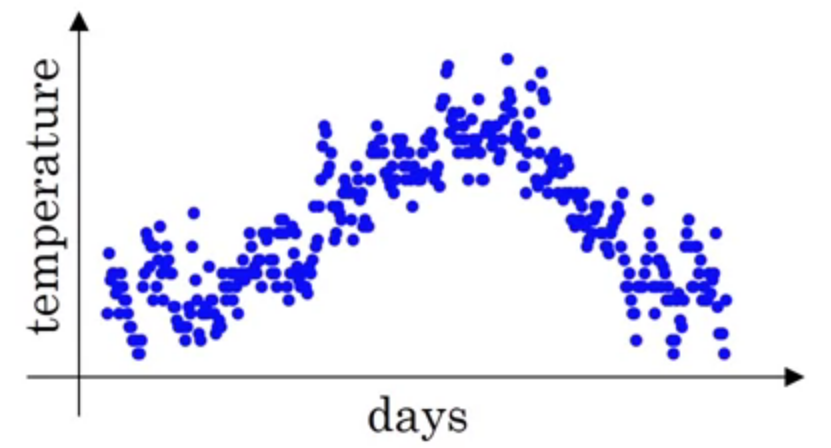
\includegraphics[scale=0.4]{Res/temperatures-london.png}
\label{temperatures-london.png}
\end{figure}

Here we sse that the values are very noisy, going up and down on each day.
However, if we want to visualize the \textit{trend} of the values, we can apply
the moving average technique.

Basicaly, instead of plotting these points (let's call them $\theta_i$), we'll
plot $V_i$.

First, we initialize $V_0$ as zero.
\[
V_0=0
\]

then, we get the next value by averaging the previous value of $V_i$ and the
current value of $\theta_i$.
\[
V_1=0.9V_0+0.1\theta_1
\]
a general formula would be:
\[ \boxed{
    V_i = 0.9V_{i-1}+0.1\theta_i
}\]

If we compute and plot that, we'll get figure \ref{temperature-average.png}

\begin{figure}[h]
\centering
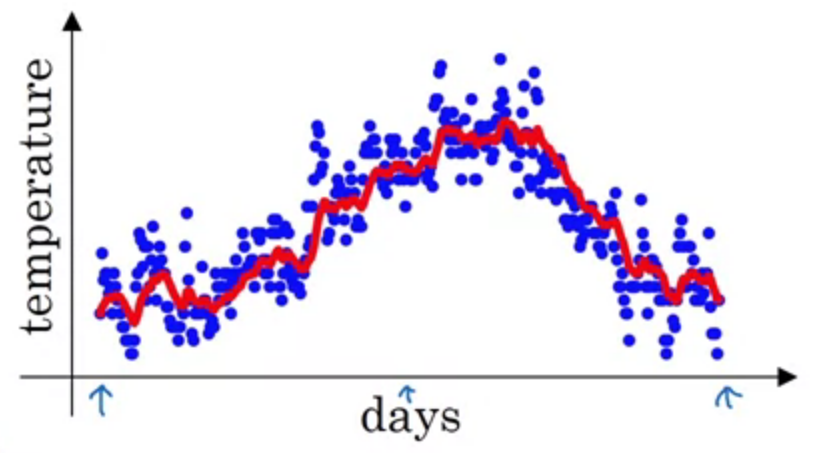
\includegraphics[scale=0.4]{Res/temperature-average.png}
\caption{The moving average of the temperatures.}
\label{temperature-average.png}
\end{figure}

We see that we got a much more smooth curve because we're always considering the
previous value to create the next one. We could make the formula even more
general:
\[ \boxed{
        V_i=\beta V_{i-1}+(1-\beta)\theta_i
}\]

where $\beta$ is the percentage of how much we would like to consider the
previous value.

Indeed the value of $\beta$ will dictate approximately how many previous
iterations we're considering on each point. To have an idea of how many previous
points we're considering, we use the formula
\[
\dfrac{1}{1-\beta}
\]

Therefore, for $\beta=0.9$, we're considering approximately the $10$ previous
temperatures in order to get the current value. That's why it's called a
\textit{moving} average or a \textit{local} average.

The lower $\beta$ is, the less temperatures we'll be considering on each
average and, therefore, the faster those averages will change, leading to a
noiser curve, but that adapts faster. And if $\beta$ is big, we'll be
considering more days and, therefore, the average will change more slowly,
leading to a smoother curve that has some latency to adapt to new trends.

This value will be a hyperparameter in our models.

To understand a little better this algorithm, let's try to get a non-iterative
formula. We'll get something like:

\[
V_i=0.1\theta_i + 0.1\times 0.9\theta_{i-1} + 0.1\times 0.9^2\theta_{i-2} +
\cdots + 0.1\times 0.9^{k}\theta_{i-k}+\cdots
\]

So, indeed, we're calculating $V_i$ as an average of \textit{all} previous
values. But the farest the values are from the current we're calculating, the
less impact it have on the current one. Indeed, we see that the influence decays
\textit{exponentially} (that's why this term apears in the name).

If we sum all coeficients, we would except to get exactly $1$, since this is an
average. But unfortunatelly, that's not what happens. In fact, we say that this
is approximately an average, because we're missing an \textbf{bias term}.

However, using this kind of average is very good computacionally, because we
don't have to keep track of (say) the last $n$ terms to compute a local average.
We can do that in $O(1)$ for each element.

If we would implement this algorithm, it would be like:

\begin{algorithm}[Exponentially weighted averages]
$V_\theta = 0$ \nl
Repeat \{ \nl
\t $V_\theta := \beta V_\theta + (1-\beta)\theta_t$ \nl
\}
\end{algorithm}

As one can see, this algorithm is very memory and time efficient.

Finally, we can make a correction to the bias term by dividing $V_i$ by
$1-\beta^{i}$.

So we can use the formula:
\[
    V_i = \dfrac{\beta V_{i-1} + (1-\beta)\theta_i}{1-\beta^{i}}
\]

This will help a lot in the first iterations where we still don't have many
values in the window. Think of it as $1-\beta^{i}$ being a good approximation
for the sum of the coefficient of the average.

\subsection{Gradient Descent with Momentum}%
\label{sub:gradient_descent_with_momentum}

The first algorithm we'll see is \textbf{gradient descent with momentum}.
Basicaly, instead of using the derivatives in each iteration, we're going to
average the derivatives using exponentially weighted averages to get a more
smooth descent to the minimum. This algorithm works pretty much always better
than normal gradient descent.

\begin{algorithm}[Gradient Descent with Momentum]
On iteration $t$: \nl
\t Compute $dW, db$ on current batch (or mini-batch) \nl
\t $V_{dW}=\beta V_{dW} + (1-\beta)dW$ \nl
\t $V_{db}=\beta V_{db} + (1-\beta)db$ \nl
\t $W=W-\alpha V_{dW}$ \nl
\t $b=b-\alpha V_{db}$ \nl
\end{algorithm}

This averaging over the last $k$ derivatives makes our algorithm take this
\textit{momentum}, which is going to create speed into the minimum direction,
avoiding oscilations in other directions like standart gradient descent does.

The downside of this algorithm is that now we have two hyperparameters instead
of just one: $\alpha$ and $\beta$. In practice, values close to $\beta=0.9$ work
good.

One more note is that in practice people tend to not use \textit{bias
correction} because after just $10$ or so iterations the algorithm will have a
very small bias value.

\subsection{RMSprop}%
\label{sub:rmsprop}

\textbf{RMSprop} which means for Root-Mean-Square prop. It also speed gradient
descent by ``normalizing'' the different directions. To do that, it takes the
element-wise square of the gradient, average it over the last $k$ squares and
than divide the gradient by the squareroot of that.

\begin{algorithm}[RMSprop]
On iteration $t$: \nl
\t Compute $dW, db$ on current batch (or mini-batch) \nl
\t $S_{dW}=\beta V_{dW} + (1-\beta)dW^2$ \nl
\t $S_{db}=\beta V_{db} + (1-\beta)db^2$ \nl
\t $W=W-\alpha \dfrac{dW}{\sqrt{S_{dW}+\epsilon}}$ \nl
\t $b=b-\alpha \dfrac{db}{\sqrt{S_{db}+\epsilon}}$ \nl
\end{algorithm}

The $\epsilon$ value here is just to garantee we're not dividing by zero.

\subsection{Adam}%
\label{sub:adam}

\textbf{Adaptative moment estimation} optimization algorithm will basicaly take
the two previous ideas (momentum and rmsprop) and put them together. It's one of
the best algorithms known so far along RMSprop.

\begin{algorithm}[Adam]
$V_{dW}:=S_{dW}:=V_{db}:=S_{db}:=0$ \nl
On iteration $t$: \nl
\t Compute $dW, db$ on current batch (or mini-batch) \nl
\t $V_{dW}=\beta_1 V_{dW} + (1-\beta_1)dW$ \nl
\t $V_{db}=\beta_1 V_{db} + (1-\beta_1)db$ \nl
\t $S_{dW}=\beta_2 V_{dW} + (1-\beta_2)dW^2$ \nl
\t $S_{db}=\beta_2 V_{db} + (1-\beta_2)db^2$ \nl
\t $V_{dW} = \dfrac{V_{dW}}{1-\beta_1^{t}}$ \nl
\t $V_{db} = \dfrac{V_{db}}{1-\beta_1^{t}}$ \nl
\t $S_{dW} = \dfrac{S_{dW}}{1-\beta_2^{t}}$ \nl
\t $S_{db} = \dfrac{S_{db}}{1-\beta_2^{t}}$ \nl
\t $W=W-\alpha \dfrac{V_{dW}}{\sqrt{S_{dW}+\epsilon}}$ \nl
\t $b=b-\alpha \dfrac{V_{db}}{\sqrt{S_{db}+\epsilon}}$ \nl
\end{algorithm}

So as one can see, we're basicaly doing what we're doing in RMSprop, but now
instead of using $dW,db$, we're using the average over the last $k$ values, just
like in momentum.

One more thing here is that we're using bias correction, which is very common to
do in this algorithm.

Now we have three hyperparameters: $\alpha,\beta_1,\beta_2$. In practice,
$\alpha$ still needs to be tuned, and common values for the other two are
$\beta_1=0.9$ and $\beta_2=0.999$. There's also the value of $\epsilon$, but
this is very rare to chance. We usually use something like $\epsilon=10^{-8}$.

\subsection{Learning Rate Decay}%
\label{sub:learning_rate_decay}

One more technique that can be used through all the optimization algorithms is
\textbf{learning rate decay}. Basicaly, we slowly reduce the $\alpha$ parameter
in our algorithm by the time. In the begining, we're far alway from the minimum,
so we can set our learning rate higher and as we go towards the minimum, we
reduce this learning rate to make it smaller and more precise. One way to do
that, is to use the formula:

\[
\alpha=\dfrac{1}{\text{decay\_rate}\cdot\text{num\_epoch}}\cdot\alpha_0
\]

Other formulas use exponentially decay:
\[
\alpha=0.95^{\text{num\_epoch}}\cdot\alpha_0
\]
\[
\alpha=\dfrac{k}{\sqrt{\text{num\_epoch}}}\cdot\alpha_0
\]

\section{Hyperparameter tuning}%
\label{sec:hyperparameter_tuning}

We've seem so far that the algorithms have lots of hyperparameters to turn, like
the number of layers, number of nodes in each layer, mini-bath sizes, $\alpha$,
$\beta_1$, $\beta_2$. Also the decision of using one optimization algorithm
instead of other could be considered as a hyperparameter.

We need to understand how to select the values of the hyperparameters we're
going to try. In the early machine learning times, we used a grid to try the
hyperparameters. For instance, if we had $h_1$ and $h_2$, than we would say in
each values of them we wanted to try. Let's say we want to try
$h_1=\set{v_1,v_2,v_3}$ and $h_2=\set{u_1,u_2,u_3}$. Them we would try all the
combinations of these values:
\[
    h_1\times h_2=\set{(v_1,u_1),(v_1,u_2),\cdots,(v_3,u_3)}
\]

This is good when the number of parameters is small. But in deep learning, the
number of parameters tend to be large and, thus, we use random points (i.e., for
each hyperparameter, we pick a random value in some region).

\begin{figure}[h]
\centering
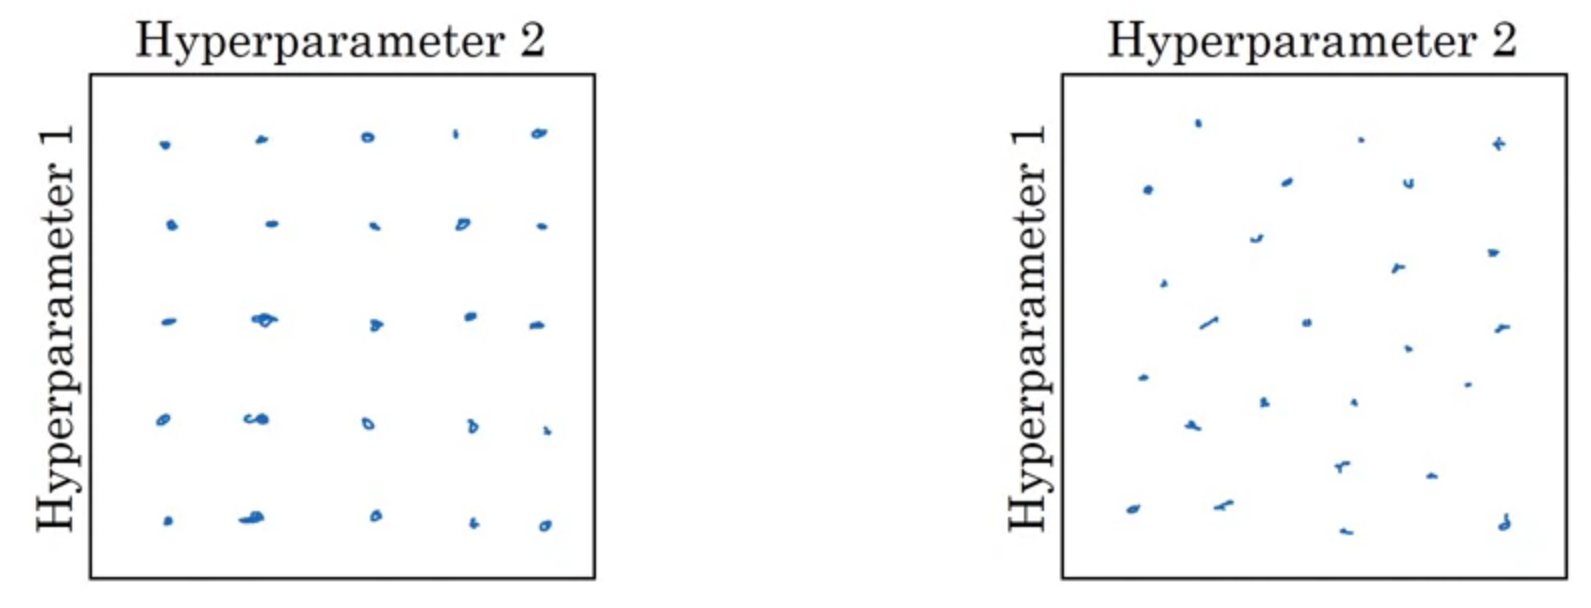
\includegraphics[scale=0.4]{Res/hyperparamter-search.png}
\caption{In the left we see the Grid Search and in the right, we see the random
search}
\label{hyperparamter-search.png}
\end{figure}

Another good thing to do is to perform many hyperparameter searchs. In the first
one, we can use larger scales for each hyperparameter and discover that the best
value for, let's say, $\alpha$ is between $0.9$ and $1.1$. Than we can perform a
new search sampling values of $\alpha$ just in that region and discover that the
best value is approximately $0.96$.

\subsection{Selection the appropriate scale for hyperparameters}%
\label{sub:selection_the_appropriate_scale_for_hyperparameters}

In many cases, we don't want to \textit{uniformily} sample values from a
particular range. Suppose we use the range $\sbracket{0.0001, 1}$ for the
learning rate $\alpha$. Then it's clear that most ($90\%$) of the time we'll
select values between $0.1$ and $1$. That's not what we want. We want, to select
values between $(0.0001,0.001)$, $(0.001,0.01)$, $(0.01, 0.1)$ and $(0.1,1)$ in
the same proportion.

Therefore, what we need to do is to sample using a \textit{logarithmic} random
scale.

To do that in python, one way is the following:
\begin{lstlisting}[language=python]
r = -4 * np.random.rand()
alpha = 10 ** r
\end{lstlisting}

\paragraph{Scale for parameter $\beta$}%
\label{par:scale_for_parameter_beta_}

Another important topic is how to pick a scale for the parameter $\beta$. We've
seem that $\beta=0.9$ means we're averaging over the $10$ previous gradients and
if $\beta=0.999$, we're averaging over the last $1000$ gradients. So we want to
have a linear sample \textit{in the number of gradients}. To do that, we can
think in $1-\beta$ and get the interval $(0.1, 0.001)$. And just like in the
example from above, we can use a logarithmic scale, but now reversed. Therefore,
we use:
\[
\beta=1-10^{r}
\]

Instead of the code above.

\section{Batch normalization}%
\label{sec:batch_normalization}

As we've seem before, input normalization can help a lot to optimize our
algorithm and train faster. Another technique is called \textbf{batch
normalization} in which normalize the values in between the hidden layers.

So basicaly for each intermediate value $\xlayer[z]{l}$, we normalize it using:
\[
\mu=\dfrac{1}{m}\spsum{i}{}\xlayer[\xii[z]{l}]{i}
\]
\[
    \sigma^2=\dfrac{1}{m}\spsum{i}{}\paren{\xlayer[\xii[z]{l}]{i}-\mu}^2
\]
\[
\xlayer[\xii[z]{l}]{i}_{\text{norm}}=\dfrac{\xlayer[\xii[z]{l}]{i}-\mu}
{\sqrt{\sigma^2+\epsilon}}
\]

But indeed, we don't want all the intermediate values to be normalized, so we
do:
\[
\xlayer[\xii[\tilde{z}]{l}]{i}=\gamma\xlayer[\xii[z]{l}]{i}_{\text{norm}}+\beta
\]

where $\gamma$ and $\beta$ are learnable parameters of the model (using their
gradient as with $W$ and $b$).

This allows us to change the mean and variance of each layer to our benefit.

Basicaly now, instead of doing this process:
\[
    X
    \xrightarrow{\xlayer[W]{1},\xlayer[b]{1}}\xlayer[z]{1}
    \xrightarrow{\xlayer[g]{1}}\xlayer[a]{1}
    \xrightarrow{\xlayer[W]{2},\xlayer[b]{2}}\xlayer[z]{2}
    \xrightarrow{\xlayer[g]{2}}\xlayer[a]{2}
    \rightarrow\cdots
\]

We're doing:
\[
    X
    \xrightarrow{\xlayer[W]{1},\xlayer[b]{1}}\xlayer[z]{1}
    \xrightarrow{\xlayer[\gamma]{1},\xlayer[\beta]{1}}\xlayer[\tilde{z}]{1}
    \xrightarrow{\xlayer[g]{1}}\xlayer[a]{1}
    \xrightarrow{\xlayer[W]{2},\xlayer[b]{2}}\xlayer[z]{2}
    \xrightarrow{\xlayer[\gamma]{2},\xlayer[\beta]{2}}\xlayer[\tilde{z}]{2}
    \xrightarrow{\xlayer[g]{2}}\xlayer[a]{2}
    \rightarrow\cdots
\]

And we can compute the gradient of all parameters to update each of them using
Gradient Descent.

\begin{obs}
    We also need to say that indeed, when using batch normalization, we don't
    need to use the $b$ parameter at all, because $\beta$ will always change it
    before computing $a$. Therefore, the only parameters we need are
    $W,\gamma,\beta$.
\end{obs}

\section{Multiclass problems}%
\label{sec:multiclass_problems}

So far, we've seem only how to do binary classification with neural nets. Now,
let's see a logistic regression variatiante that allow us to have multiple
classes: \textbf{softmax regression}.

\begin{nota}
\begin{itemize}
    \item $C$ will denote the number of classes;
    \item The classes will be numbers from $0$ to $C-1$.
\end{itemize}
\end{nota}

The first modification we'll do is in the output layer. Now $\hat{y}$ will be a
vector instead of a single number and $\hat{y}_i = p(i\cond x)$, i.e., the
probability of class $i$ given the input $x$.

We'll use an \textbf{softmax} layer in the output layer to achive such goal. To
do so, we'll compute $\xlayer[z]{L}$ as usual and use the \textbf{softmax
activation function}, which is:

\begin{align*}
    t &= e^{(\xlayer[z]{L})} \\
    \hat{y}=\xlayer[a]{L} &= \dfrac{e^{(\xlayer[z]{L})}}{\spsum{i}{}t_i}
\end{align*}

As you can see, we basicaly compute this vector $t$ and divide by the sum of its
components (it's like we were normalizing $t$).

Indeed, if we sum the coordinates of $\hat{y}$, they'll add up to $1$.

\section{Deep Learning Frameworks}%
\label{sec:deep_learning_frameworks}

We've learned so far how to program deep learning algorithms from scratch but
there are several python frameworks that are used in practice when implementing
these deep learnings algorithms.

Some of the most used DL frameworks are:
\begin{itemize}
    \item Keras
    \item TensorFlow
    \item Torch
\end{itemize}

%%%%%%%%%%%%%%%%%%%%%%%%%%%%%%%%%%%%%%%%%%%%%%%%%%%%%%%%%%%%%%%%%%%%%%%%%%%%%%%%

\chapter{Machine Learning Projects}%
\label{cha:machine_learning_projects}

In this chapter, we're going to focus on how to structure our machine learning
projects so that we don't waste a lot of time (say) colleting data when the
bottleneck say the number of layers or not regularizing.

\section{Setting up your goal}%
\label{sec:setting_up_your_goal}

One of the first things we need to set up is a \textbf{single real value} as a
metric goal. By donig this, one can evaluate the model and have a clear goal
(improve $x\%$ of that metric).

Also, sometimes we want to restric our model to certain conditions like
\textit{running time}, we want it to be low. So we would just really care about
our model it is runs in less than (say) $100$ ms. This kind of metric is called
an \textbf{satisficing} metric, while the real value we said before is called an
\textbf{optimizing} metric.

We want to maximize (or minimize) the optimizing metric under the condition
given by the satisficing metric.

All these metrics must be calculated under a training set, or evaluation (dev)
set or testing set. So let's talk a little about how to set these sets.

Basicaly, the gold rule for when spliting the sets is to keep the same
distribution in each one of them. If we have data of pictures of cats tha come
from cellphone, regular cameras and profisional cameras, we want to have the
same percentage of each of these types through all sets.

\paragraph{When to change the evaluation metric?}%
\label{par:when_to_change_the_evaluation_metric}

Let's suppose that we have two algorithms A and B with $3\%$ and $5\%$
classification errors respectively, but suppose that algorithm A is classifing
wrongly photos of pornograph as photos of cats and would show it to the
customers, which is a massive error to our company. Therefore, we prefer
algorithm B even if it missclassifies more.

When things like this happen, we need to either change our evaluation metric or
change our dev and training sets to adapt to the kind of error we're having. One
example is weighting the examples to make porn pictures have a very large error
while non-porn pictures have a normal error.

\section{Comparing to humam-performance}%
\label{sec:comparing_to_humam_performance}

One of the things we should aim when using a machine learning system to
accomplish a certain goal is to check how well humans perform that goal. By
doing this we can have a kind of standard line of what is a good or bad model. A
good model is one that does the task better than us humans.

When we look at the graph of accuracy of models over time, we see that it's very
easy to surpass the human level of performance and than it starts to slow down
the increase in performance until is barly reaches the maximum amount of
performance, which is called the \textbf{Bayes optimal error}, which is a
theorical best possible error.

\begin{figure}[h]
\centering
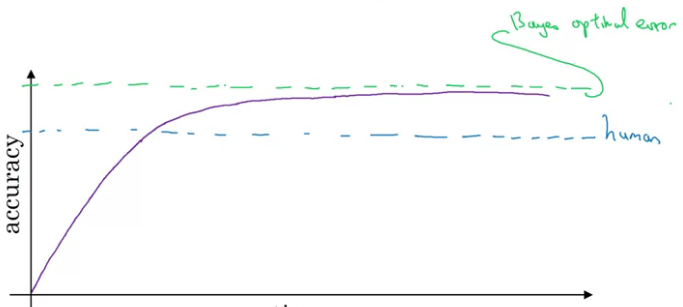
\includegraphics[scale=0.6]{Res/human-performance.png}
\caption{}
\label{human-performance.png}
\end{figure}

One nice trick that we can use for tasks that humans are good at is to use
specific knowladge to see where the model are is getting things wrong and try to
get more labeled examples for that situation in order to help the model. We also
can look at the missclassified examples to check if the algorithm have a high
bias or high variance.

\paragraph{Avoidable bias}%
\label{par:avoidable_bias}

Understanding human level of performance is also important because we can
estimate the bayes optimal error. If we know that humans have $1\%$ of error and
our algorithm has $8\%$ of error in the training set and $10\%$ in the dev set,
then we should try to reduce bias to achieve something closer to $1\%$.
Meanwhile, if our algorithm had $1.5\%$ in the training set and $3\%$ in the dev
set, then we should concentrate in reducing variance to make the $3\%$ closer to
$1.5\%$.

\paragraph{How to define human-level error/performance}%
\label{par:how_to_define_human_level_error_performance}

Let's say we have medical pictures to give a certain diagnostics. Then, to
define human-level of error, we should get the best possible team of experienced
doctors to discuss the pictures and give their opinions on that picture. The
error that those people have will be lower than a typical doctor or a single
experienced doctor. Therefore, we use this error as the goal.

\section{Error Analysis}%
\label{sec:error_analysis}

When we're trying to create an algorithm that does some kind of human task,
manually checking the errors our algorithm is making can give us some insights
of how to improve. This is called \textbf{error analysis}.

One of the most simples things we can do in error analysis is check what are the
classes that a classifier is mostly making mistakes. Than, we could focus on
getting more examples of that class.

Another example could be the case where many images with a white background are
being missclassified. Thus, it could be a good ideia to collet more images with
white background and train on those images.

If we have some high percentage of error for many different kinds of imagens, we
could also evaluate all those ideas im parallel, with many teams working on
those different kinds of errors and trying to improve them.

\paragraph{Incorrectly Labeled Data}%
\label{par:incorrectly_labeled_data}

In many cases, our algorithm can perform some errors because the training data
itself has some misslabed examples. What should we do when we encounter that?

The first thing to say is that DL algorithms are quite robust to random errors
in the trainig set. If the erros are quite random, then it's oks to leave them
as they are because this is probably not going to affect much the outputs.
However, if the error has a bias (i.e., it's not random), then we definitely
should fix those incorrectly labeled examples.

For instance, if all white dogs are labeled as cats, them our algorithm will
learn to classify white dogs as if they were cats.

When doing error analysis, we create a table where the lines are the
missclassified examples and the columns are the possible errors associated with
that particular example. Then, we sum up all the ``checks'' in each column and
see which errors are the most crucial to our application. If incorrectly labeled
data is one of those things, we might add a column to check when that instance
was misslabeled and, if at the end, there were a lot of them, we might separete
a team to work on fixing those labels.

\paragraph{Iterating}%
\label{par:iterating}

One important thing to do then building a machine learning project is to first
build it quickly and them use error analysis to avaluate your model and improve
it. After knowning where to improve, to that and repeat everything again.

\section{Mismatched Training and Dev/Test Sets}%
\label{sec:mismatched_training_and_dev_test_sets}

In many cases, teams building Deep Learning systems just throw a bunch of
instances into the training set to make it better. And in many of these
situations, the training and dev/test sets will end up with different
distributions. So how to deal with those cases?

Suppose we have pictures of cats and $200,000$ of them come from the web, have a
high resolution, where taken by professionals while just $10,000$ of them come
from mobile app, by amartures that will use our app to predict if the image is a
cat or not.

Our final user will input a regular image, taken by a phone, while our main
source of imagens aren't like that. So what do to?

\textbf{Option 1} is to just mix these two kinds of imagens and shuffle them
around the training, dev and test sets. Now we do have the same distribution of
pictures, but we'll end up with a very small proportion of mobile photos in our
dev and test sets, which is not what we want at all.

\textbf{Option 2} is to just put all the imagens from the web into our training
set together with some of the mobile images and leave the rest of the mobile
images into the dev and test sets (so they'll end up with no web images).
Suppose we use all the $200,000$ images from the web into the training set and
add up more $5,000$ images from the mobile app, while the dev and testing set
will have $2,500$ images from the mobile app each.

\paragraph{Bias and Variance}%
\label{par:bias_and_variance}

One thing to notice is that bias and variance analysis will be different if we
have mismatched training and dev/test sets. Before, we knew that if the training
error is $1\%$ and the dev error is $10\%$, them we have a large variance and
probably the algorithm is overfitting. But if the training and dev data come
from different distributions, we can no longer say that. Maybe the dev set just
has poor quality images and it's harder to predict them, we don't know.

In order to accomplish this error, we can create a new set of data that we'll
can it the \textit{training-dev set}, which has the same distribution of the
training set, but it's not used for training. Now we use the training-dev to
check problems like bias and variance and if it's ok, we know that the $10\%$ is
just from the data mismatch.

\paragraph{Addressing Data Mismatch}%
\label{par:addressing_data_mismatch}

We've seem that creating a training-dev set can show us the amount of error we
have due to data mismatch from the training and dev/test sets. So how to address
that in order to reduce this error? Indeed there are not automatic ways to do
that, but we can look at a few things.

One possible thing is to carry out manual error analysis to try to udnerstand
difference. Than, we would try to make the training data more similar, or
collect more data similar to dev and test sets. For instance, we could try to
make the images of the cats more blury, or low resolution.

\section{Transfer Learning and Multi-Task Learning}%
\label{sec:transfer_learning_and_multi_task_learning}

In many cases, we can use a NN trained in some task to improve another NN in
other task, that's called \textbf{transfer learning}. Let's see how to do it.

Suppose we have a NN to make image recognition and want to do radiology
diagnosis. What we could do it just delete the last layer of the NN (the output
layer) and randomly initialize a new output layer for the new task.

By doing this, we hope that when the NN learned about how to recognize imagens,
it already may know how to recognize parts of images to help us in the
diagnosis.

Another example could be a NN for speech recognition and we want a system for a
trigger word. We can add several new layers and just train them, or we can train
the whole network, but starting with the pre-trained weights.

Transfer learning is useful when we have a pre-trained model that was trained
with lots of data, but we're trying to solve a problem that has a small
dataset. \jump

What we could also do is try to learn from multiple tasks. That's called
\textbf{multi-task learning}. Usually we use this kind of learning when we have
a NN that is trying to do many things at the same time. For instance, if we have
an autonomus car that detects pedestrians, cars, stop signs, traffic lights,
etc. Then we could train a single NN that have a large output that predicts all
thoses things at the same time. By doing this, we hope that learning one of
those things will help to learn the others and lead to a better performance
(that's what usually happen in practice).

Multi-task learning is useful when we have similar tasks that can benefit from
each other and when we have pretty much the same amount of data for each task.

\section{End-to-End Deep Learning}%
\label{sec:end_to_end_deep_learning}

In many applications, we have a pipeline with many different stages until we
reach a final result. For instance, in speech recognition, we may have to
transform the audio into some set of features that will be transformed into
phonemes that will be transformed into words that will be transformed into the
trascript.

In some cases, when we have a lot of data, we can bypass all those intermediate
steps and translate audio into text with a single NN. That's what's called
\textbf{end-to-end deep learning}.

%%%%%%%%%%%%%%%%%%%%%%%%%%%%%%%%%%%%%%%%%%%%%%%%%%%%%%%%%%%%%%%%%%%%%%%%%%%%%%%%

\chapter{Convolutional Neural Networks and Applications}%
\label{cha:convolutional_neural_networks_and_applications}

\textit{Convolutional Neural Networks} are one special kind of NNs that are
specially suited for \textit{Computer Vision} problems. Some of these problems
include:
\begin{itemize}
    \item Image classification;
    \item Object detection;
    \item Style transfer;
    \item ...
\end{itemize}

One of the most challeging facts about Computer Vision is that images can be
very large. If we have a $1000\times 1000$ image, than we have an input $3$
million variables (because there are $3$ color channels). That unquestionably
huge for a ``standard'' neural net (or what we'll call \textit{dense} NN or
\textit{multilayer perceptron} network - MLP). CNNs are suited for those tasks
because they allow us to reduce the number of parameters we would have with a
MLP.

\section{Convolution Operation}%
\label{sec:convolution_operation}

First, we need to understand the convolution operation itself (which is
independent of the concept of a neural net). To ilustrate that, we'll use the
example of \textit{edge detection}.

So suppose we want to detect vertical lines in a certain picture. One way to do
that is by creating a \textbf{filter} (also called \textbf{kernel}) which is a
$3\times 3$ matrix what we'll \textbf{convolve} that matrix with the image
matrix.

\begin{figure}[h]
\centering
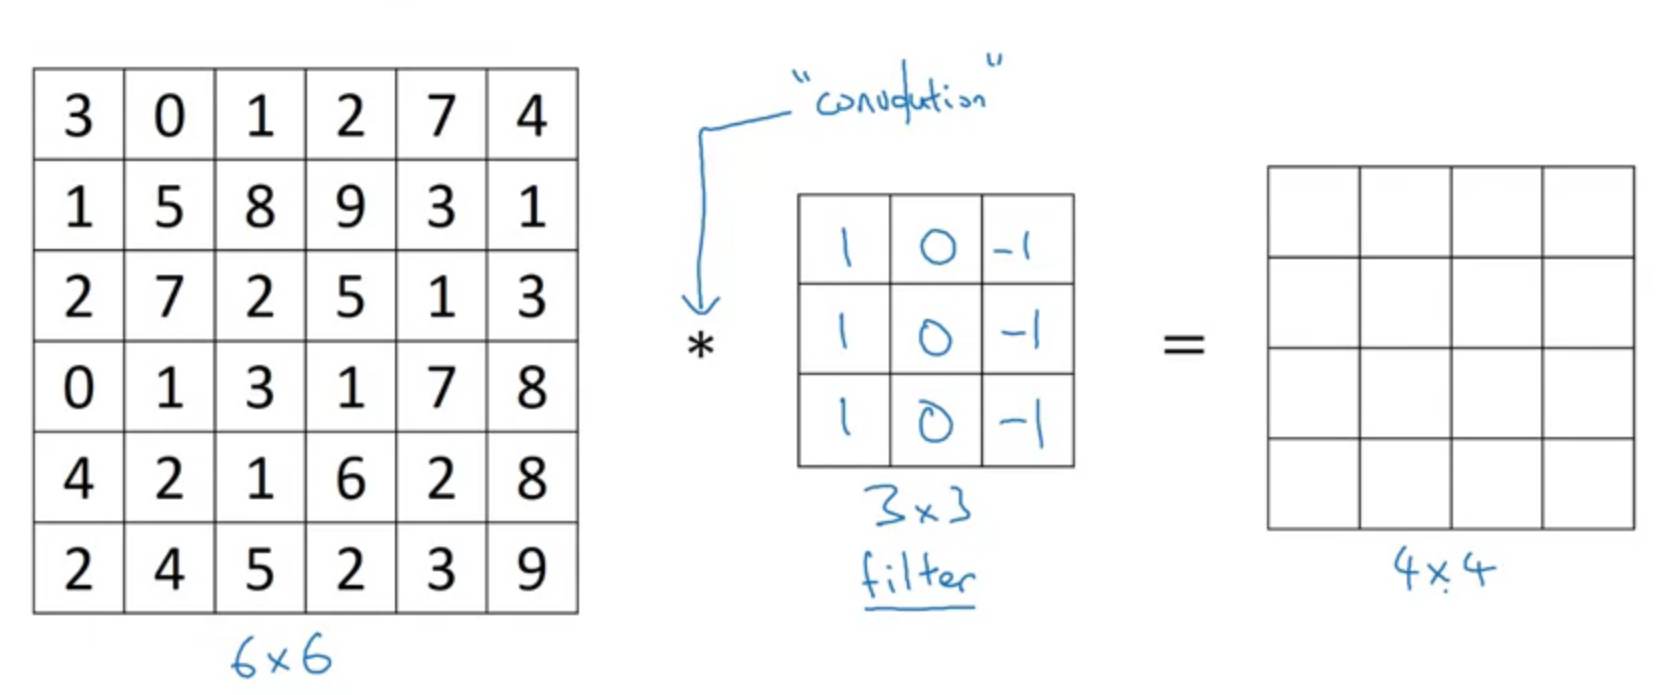
\includegraphics[scale=0.35]{Res/convolution.png}
\caption{Here we have a $6\times 6$ matrix representing an image and a $3\times
3$ filter that we'll convolve with the image resulting in a $4\times 4$, which
will be a new image.}
\label{convolution.png}
\end{figure}

The output of a convolution if given as the following (look at image
\ref{convolution.png}):

If we have a $6\times 6$ image, we'll put our filter uppon the image, one the
upper left corner. So the filter will be aligned with a $3\times 3$ submatrix of
the image. Then, we multiply the terms that are aligned and sum all of them
together to get the answer. Figure \ref{convolution-computation.png} ilustrates
this process.

\begin{figure}[h]
\centering
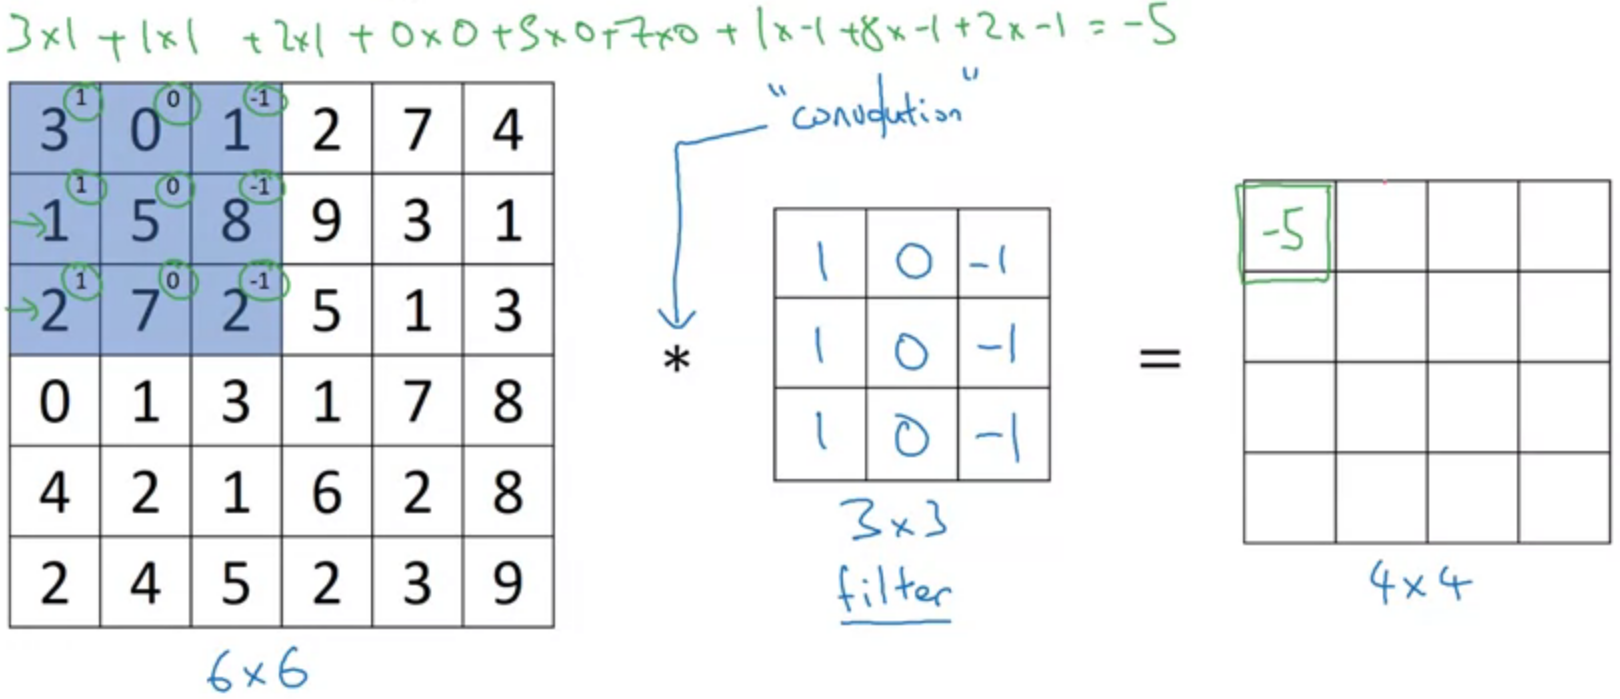
\includegraphics[scale=0.3]{Res/convolution-computation.png}
\caption{Here we see an example of how to compute the elements of the resulting
matrix.}
\label{convolution-computation.png}
\end{figure}

Then, we shift the filter one the left and compute it again until we've moved
the filter all the way through the image.

Formally, we could define it as following:

\[
    C = \paren{\spsum{l=0}{n-1}\spsum{k=0}{n-1}A_{i+k,j+l}\cdot F_{k,l}}_{i,j},
\]


where $A$ is a matrix and $F$ is a $n\times n$ filter. \jump

To understand why that $3\times 3$ matrix tells us where are the vertical edges,
we could think that it cares when we have bright pixels on the left and dark
pixels on the right, don't carring much about what's in the middle.

If we wanted to detect horizontal edges, we could use:
\[
\begin{bmatrix}
    1 & 1 & 1 \\
    0 & 0 & 0 \\
    -1 & -1 & -1 \\
\end{bmatrix}
\]

Also, there's no particular reson why we would like these particular numbers, we
could use:
\[
\begin{bmatrix}
    1 & 0 & -1 \\
    2 & 0 & -2 \\
    1 & 0 & -1 \\
\end{bmatrix}
\]

which is called the \textit{sobel filter}, or:
\[
\begin{bmatrix}
    3 & 0 & -3 \\
    10 & 0 & -10 \\
    3 & 0 & -3 \\
\end{bmatrix}
\]

which is called the \textit{scharr filter}.

We can also try to learn the filter to have a good edge detector. Indeed, it can
learn to detect $45º$ edges or $70º$ edges or whatever is better to the problem
you're trying to solve. Later in this chapter, we'll see how to make a neural
network learn these filters as parameters (but you can already see that it
reduces drastically the number of parameters we'll learn, because now instead of
having a weight for each pixel, we just have to learn these filters, which are
smaller than the original picture).

\subsection{Padding}%
\label{sub:padding}

Before we procede, we need to talk about \textit{padding}. We've seen that after
convolving those matrices, the output is \textit{smaller} than the original
input. In many applications, we don't want that, we want the output to have the
same dimentions of the original input.

Another down side of that we've been doing is the fact that the border pixels
are used way less often than the middle pixels (because there are more filter
pisitions that overlad the middle pixels).

Padding is a solution to both of those problems. Before we apply the
convolution, we pad the image, extending it with aditional zeros on the border.

Originally, if $f$ is the filter size and $n$ is the input dimension, then the
output would have $n-f+1$ dimensions. But if add an extra border (or pad) of $p$
pixels around the image, than the output dimension will be $n+2p-f+1$.

Therefore, to preserve the image dimensions, we must have $p = \dfrac{f-1}{2}$.

Indeed, the two most common type of convolutions are the ones with no padding or
the ones with a padding that leads to an output with same size as the input
(also, by convention, $f$ is usually odd). We usually called these ``valid'' and
``same'' convolutions respectively.

\subsection{Strided convolutions}%
\label{sub:strided_convolutions}

Another modification we can do to the convolutions is adding strides, which
means that we're not going to step just one to the right or one down, but more
than that. This step parameter is called the \textit{stride}.

If we say we'll have a stride of $2$, than we'll jump two squares to the left
(or down) instead of just one. That leads us to a smaller output, because we'll
be computing less times that element-wise product.

Therefore now we have three parameters: $f,p$ and $s$, the stride. If our input
has size $n$, them our output will have size equal to:
$\floor{\dfrac{n+2p-f}{s}}+1$.

\subsection{Convolutions over tensors}%
\label{sub:convolutions_over_tensors}

The final step before we apply convolutions to neural networks is learning how
they work with not just 2d matrices, but with $n$d matrices (also called
\textit{tensors}).

So let's suppose we want to convolve on RBG images. So now we have a $6\times
6\times 3$ image. To do that, we need a $3\times 3\times 3$ filter (or one
filter for each color channel). And notice that the last $3$ \textbf{must} match
the last dimention of the image.

\begin{figure}[h]
\centering
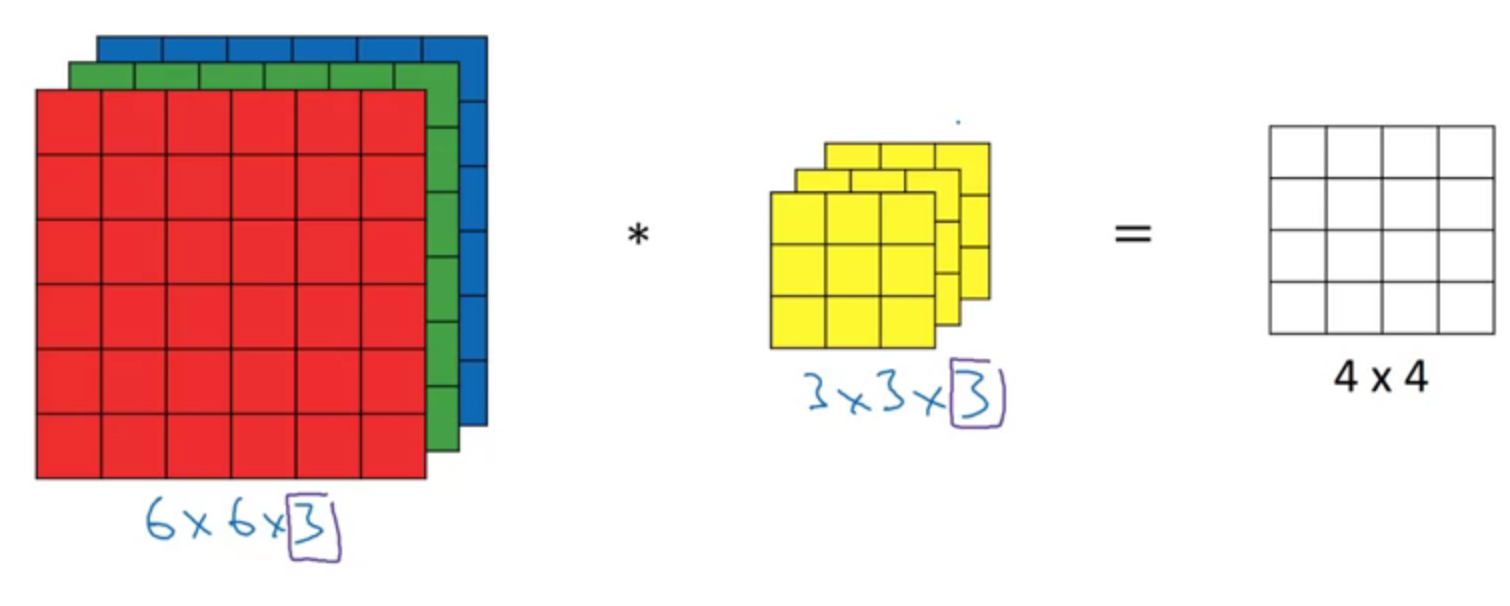
\includegraphics[scale=0.3]{Res/tensor-convolution.png}
\caption{Here we have a visualization of a tensor convolution.}
\label{tensor-convolution.png}
\end{figure}

Then the operation is very intuitive, you multiply each number of the matrix by
the coresponding number in the filter and sum all those numbers.

\section{One layers of a Convolutional Network}%
\label{sec:one_layers_of_a_convolutional_network}

Basicaly, to create a layer of a convolutional network, we need to do many
convolutions of the same previous layer (all of them with the same size). Then,
we add biases $b$ to those matrices and, finally, apply an activation function
(like ReLU or Sigmoid). The last thing we must do is stack those matrices to
create a tensor output that will be feeded into the next layer.

\begin{figure}[h]
\centering
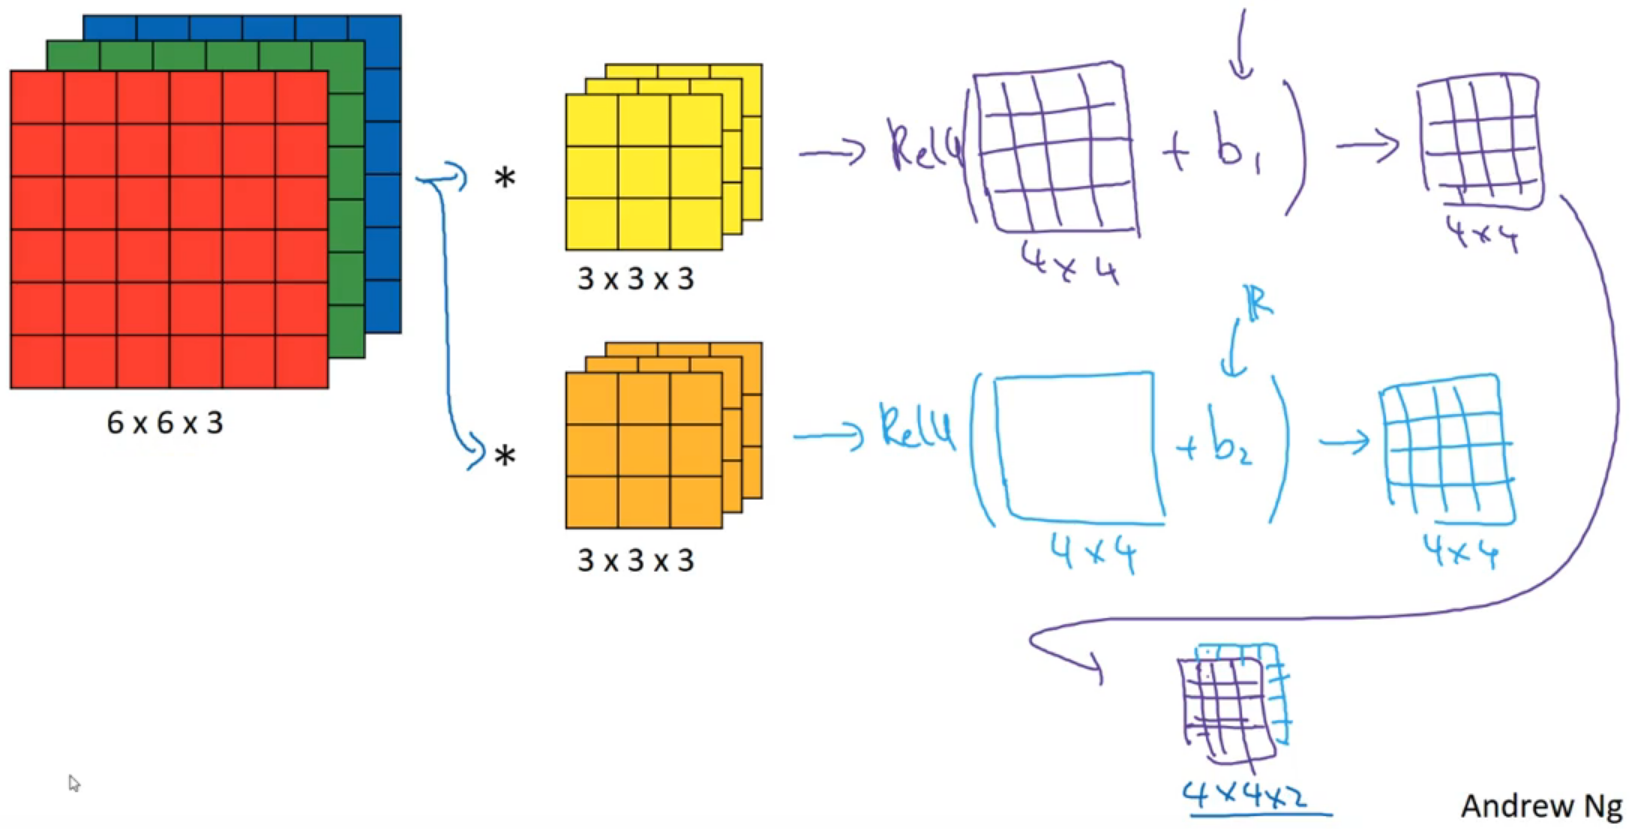
\includegraphics[scale=0.3]{Res/one-layer-convolution.png}
\caption{Here we see an ilustration of a convolutional layer.}
\label{one-layer-convolution.png}
\end{figure}

\subsection{Notation}%
\label{sub:notation}

Let's set some notation we'll be using:
\begin{itemize}
    \item $\xlayer[f]{l}$ is the filter size of the $l$-th layer;
    \item $\xlayer[p]{l}$ is the padding of the $l$-th layer;
    \item $\xlayer[s]{l}$ is the stride of the $l$-th layer;
    \item $\xlayer[c]{l}$ is the number of filters of the $l$-th layer;
    \item $\xlayer[n]{l-1}_H\times\xlayer[n]{l-1}_W\times\xlayer[n]{l-1}_c$ is
        the input shape for layer $l$;
    \item $\xlayer[f]{l}\times\xlayer[f]{l}\times\xlayer[n]{l-1}_c$ is
        the filter shape for layer $l$;
    \item $\xlayer[f]{l}\times\xlayer[f]{l}\times\xlayer[n]{l-1}_c\times
        \xlayer[n]{l}_c$ is the weights shape for layer $l$;
    \item $\xlayer[n]{l}_c$ is the bias shape for layer $l$.
\end{itemize}

\section{Pooling layers}%
\label{sec:pooling_layers}

Usually, CNNs don't have just convolutional layers (or CONV layers for short),
but can also have \textbf{Pooling layers} (or POOL layers for short) and
\textbf{fully connected layers} (or FC layers for short).

\begin{figure}[h]
\centering
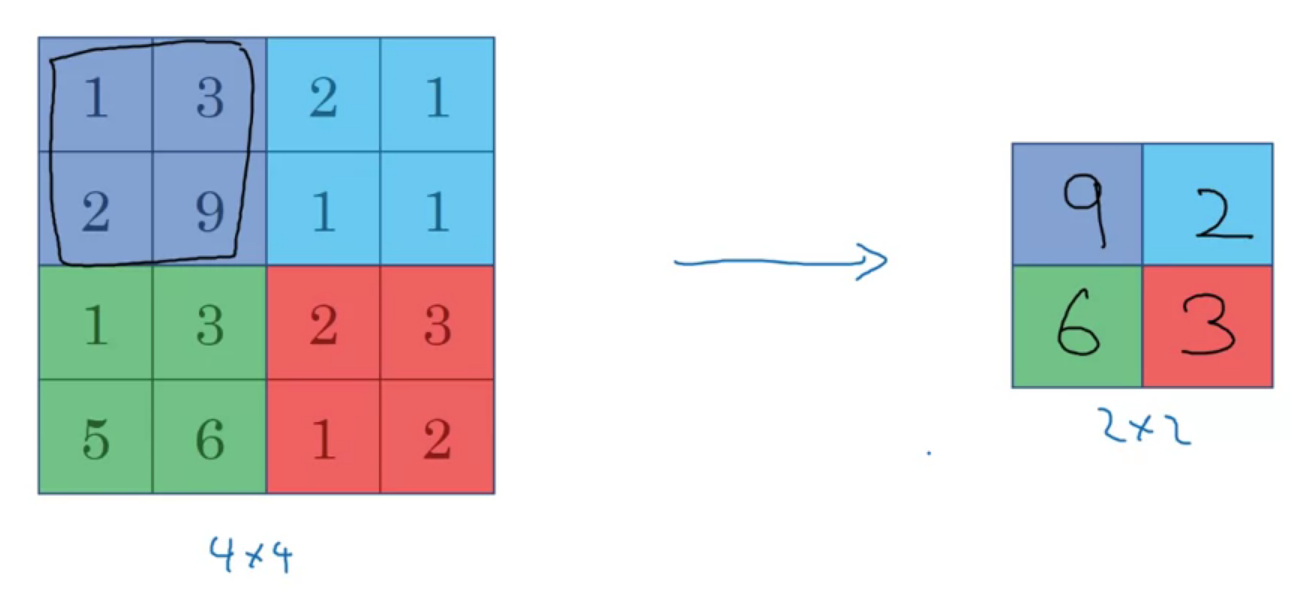
\includegraphics[scale=0.3]{Res/max-pooling.png}
\caption{An example of max pooling. This example has filter size and stride
equal to $2$.}
\label{max-pooling.png}
\end{figure}

Pooling layers are a way to speed up computations and make inputs lower. Figure
\ref{max-pooling.png} gives an example of pooling layer. Basicaly, we have that
moving window just like in convolutions, but instead of multipling and summing
the numbers, we just apply an \textbf{aggregation function} (like max, min,
prod, sum, mean, std) over those numbers.

One of the most common aggregation function is \textit{max pooling} (because
it's like we were preserving the filters were some kind of feature was
detected). But, in theory, any aggregation could be used.

Also, the concepts of stride, padding and filter size are the sames here, since
we have a moving filter.

\section{Case Studies and Classic Networks}%
\label{sec:case_studies_and_classic_networks}

In this section, we're going to study some classic convolution networks to see
why they're good and how to join the building blocks we've seem so far.

\subsection{Classical Networks}%
\label{sub:classical_networks}

\paragraph{LeNet-5}%
\label{par:lenet_5}

This network was made to recognize $32\times 32\times 1$ handwritten digits.

\begin{figure}[h]
\centering
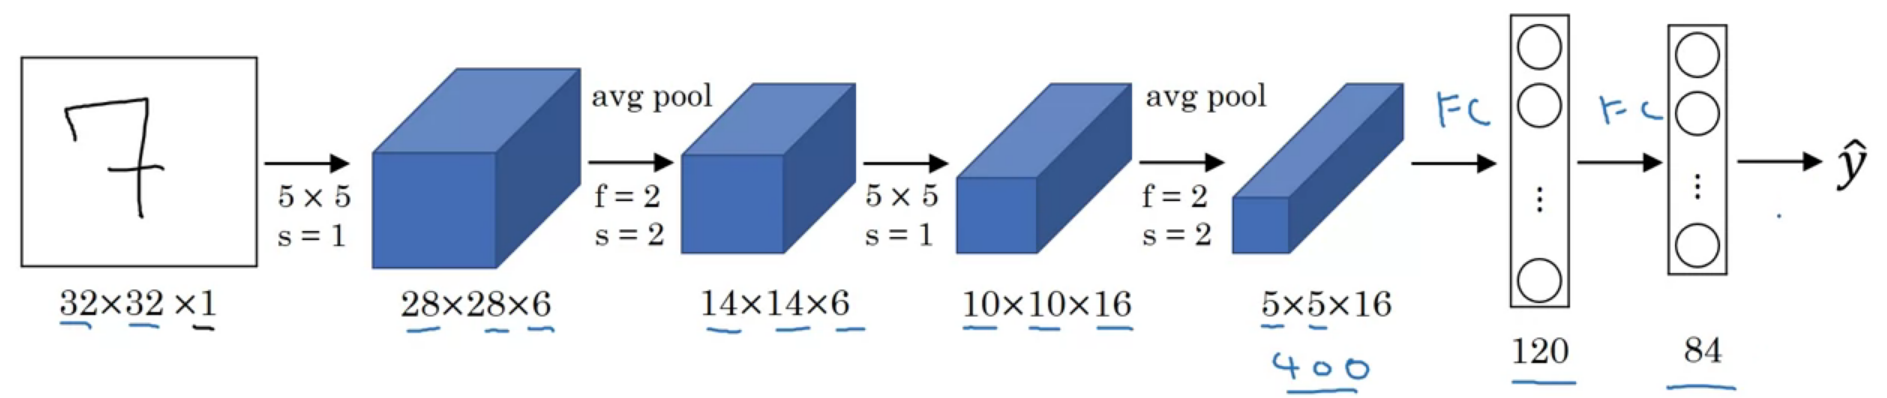
\includegraphics[scale=0.3]{Res/LetNet5.png}
\caption{Here we see the architecture of LeNet-5. At that time, we used more avg
pooling than max pooling.}
\label{LetNet5.png}
\end{figure}

It was a very small network, with $60$k parameters.

We see that it decreases the first and second dimensions and increases the
number of channels. Also it starts by interchanging pooling and conv layers and
ends with some fc layers.

\paragraph{AlexNet}%
\label{par:alexnet}

This networks was made to work with $227\times 227\times 3$ images.

\begin{figure}[h]
\centering
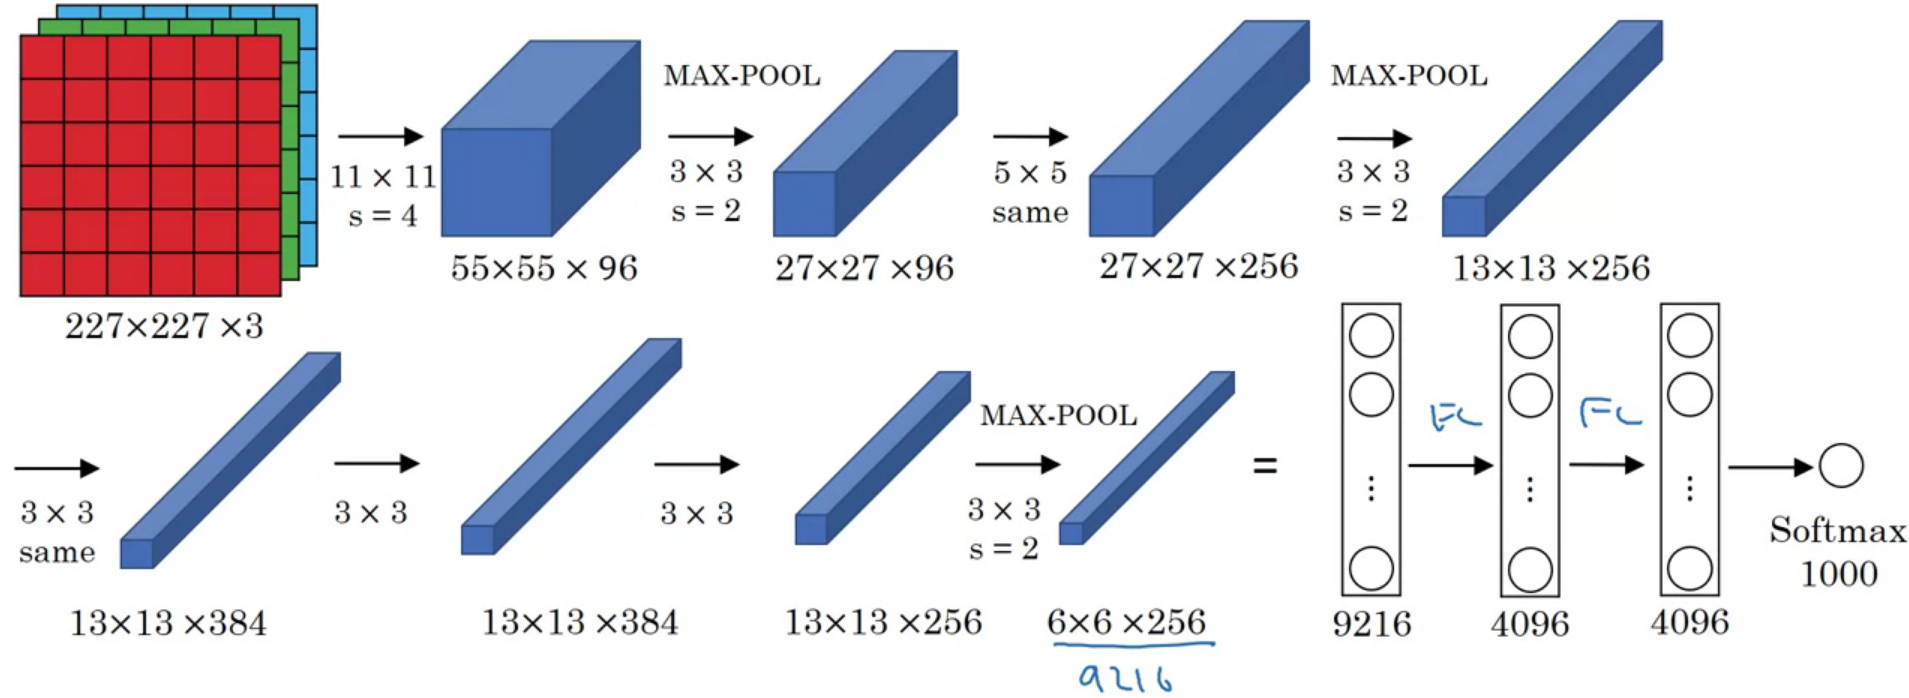
\includegraphics[scale=0.3]{Res/AlexNet.png}
\caption{Here we have a architecture of AlexNet. This is a much bigger network.}
\label{AlexNet.png}
\end{figure}

AlexNet is similar to LeNet, but much bigger, with about $60$M parameters. They
use ReLU here and Max Pooling instead of Avg Pooling.

\paragraph{VGG-16}%
\label{par:vgg_16}

Instead of using a lot of different layers with different parameters, VGG-16
uses just CONV layers with $3\times 3$ filters, stride of $1$ and same padding;
and MAX POOL layers of $2\times 2$ and $s=2$. This network is very deep, so
we're not going to draw it here.

\begin{figure}[h]
\centering
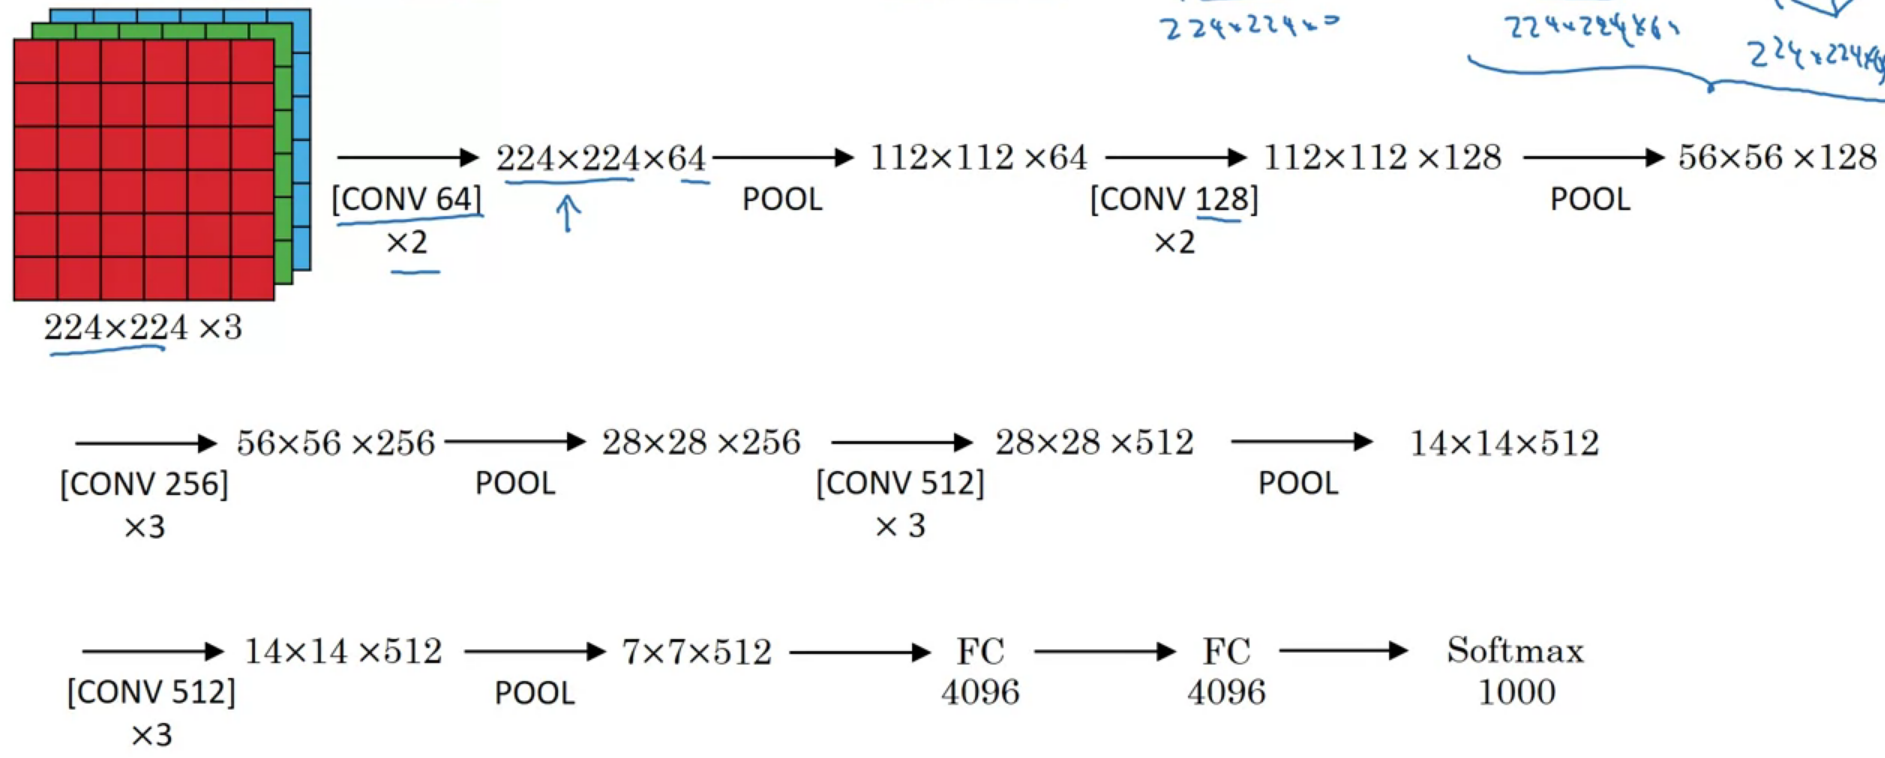
\includegraphics[scale=0.24]{Res/vgg16.png}
\caption{Here we see how big is vgg16.}
\label{vgg16.png}
\end{figure}

This network is huge, with $138$M parameters.

\subsection{Residual Networks (ResNets)}%
\label{sub:residual_networks_resnets_}

One of the most famous networks today is the Residual Network. This kind of
network use something called \textbf{skip layers}, which allow us to feed a
deeper layer with a shallow layer and skip some layers in the network. This
allow us to avoid some problems we've already mentioned such as Vanishing /
Exploding Gradients and make it possible to have networks of over 100 layers.

First, we need to understand what is a \textbf{residual block} (there's where
the name comes from).

\begin{figure}[h]
\centering
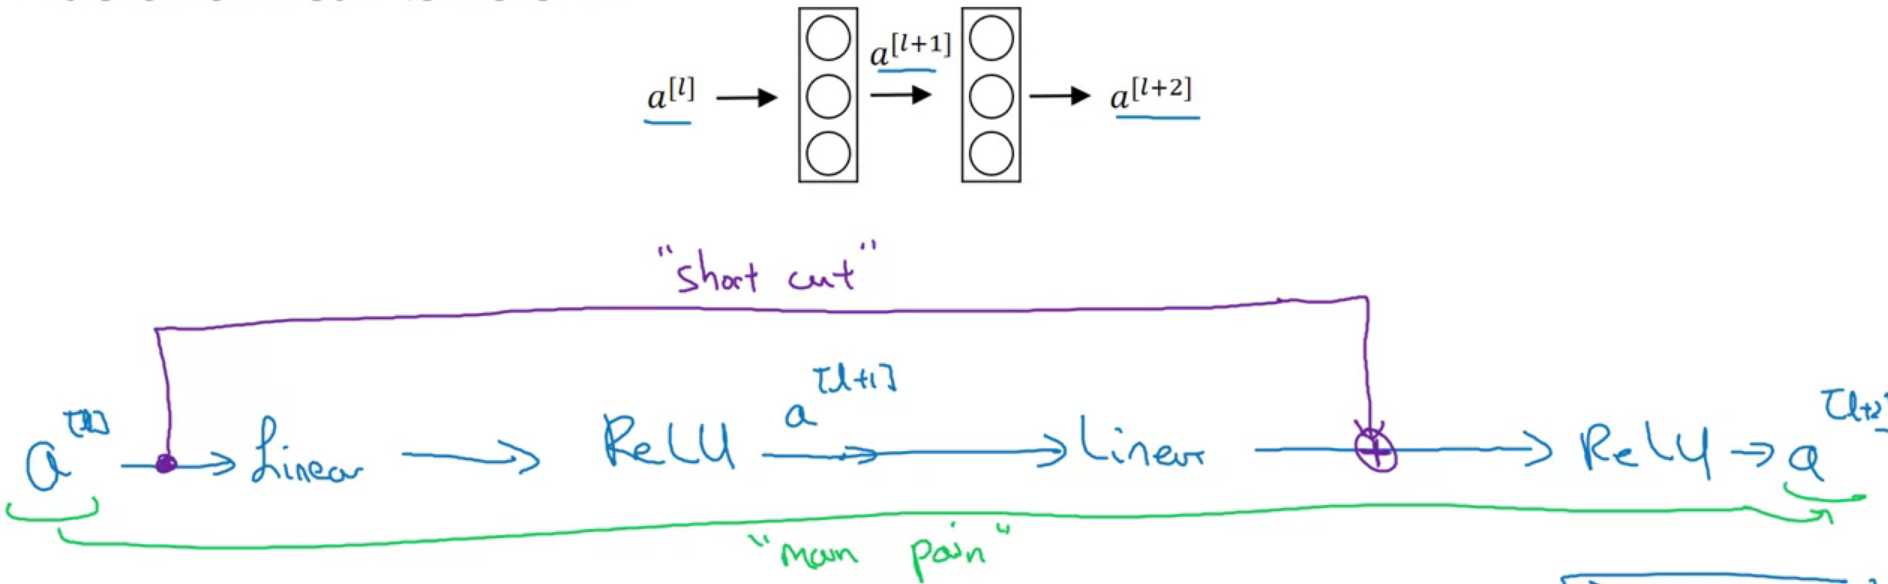
\includegraphics[scale=0.3]{Res/residual-layers.png}
\caption{Here we see an example of residual layer. Instead of following the main
path we already know, res layers allow a previous activation to \textit{short
cut} to the next layer and be added to before the ReLU of that layer.}
\label{residual-layers.png}
\end{figure}

Sometimes, we can also call these short cuts as \textit{skip connections}.

A ResNet is just a Neural Net with lots of these skip connections. In practice
we noticed that this kind of connections allowed to train for much longer,
keeping decreasing the error.

\subsection{Inception Network}%
\label{sub:inception_network}

\paragraph{$1\times 1$ convolutions}%
\label{par:_1times_1_convolutions}

First let's take a look at $1\times 1$ convolutions. You might think this is
just multiplying by a number, but it's not quite that. Suppose you have a
$32\times 32\times 192$ layer and you want to shirking it to a $32\times
32\times 32$ layer. How to do that?

One way is using $1\times 1$ convolutions. Basicaly we use $32$ $1\times
1\times 192$ filters. What these filters do is multiply all the numbers in the
``$z$'' coordinate together and output them into some activation function. So
it's like we were passing those numbers into a FC layer and outputing the next
layer.

\begin{figure}[h]
\centering
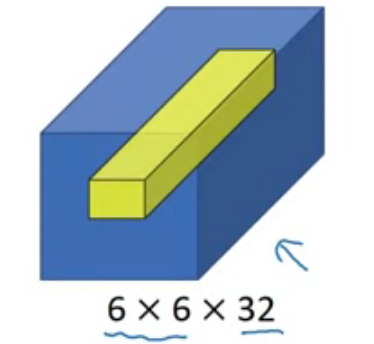
\includegraphics[scale=0.3]{Res/1x1-conv.png}
\caption{A $1\times 1$ convolution filter ilustrated.}
\label{1x1-conv.png}
\end{figure}

\jump

Inception networks use \textit{different} filters in the same layers and stack
the results in the output.

\begin{figure}[h]
\centering
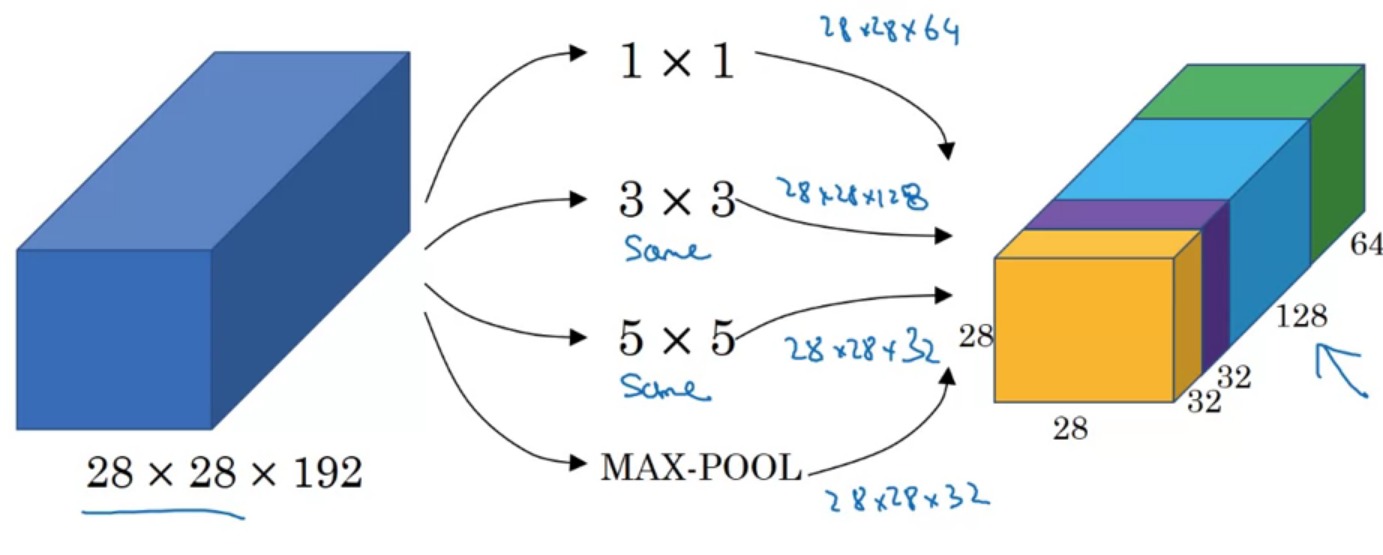
\includegraphics[scale=0.4]{Res/inseption-layer.png}
\caption{Here we see an example of inseption layer, where we apply different
filters in the same layer.}
\label{inseption-layer.png}
\end{figure}

\section{Data augmentation methods}%
\label{sec:data_augmentation_methods}

Data augmentation is the technique when we create new instances based on the
instances we already have. This technique allows us to have ``more'' data to
train, although we're not really grabbing more data.

The positive points are that you can have more instances with very little cost,
but the down side is that you might be overfitting that particular kind of data,
so it must be done with caution.

Let's explore some methods os data augmentation when applied to computer vision
(i.e. images).

\begin{itemize}
    \item The most common method is \textit{mirroring} the image;
    \item We can also take \textit{random crops} of the image;
    \item \textit{Rotation} is another technique;
    \item \textit{Shearing};
    \item \textit{Local warping};
    \item Another kind is \textit{color shifting}, in which we change the colors
        a little to make it color resilient (one can use PCA in order to find
        out which colors change more or less);
\end{itemize}

\section{Object Detection}%
\label{sec:object_detection}

Now we're going to learn how to detect object on the image. In object detection,
we want to localize potentially several objects on an image, which is different
from classifing whether an object is or not on that image.

Before moving on detection problem where we might have several objects, we'll
try a simpler problem called \textit{classification with localization}, where we
classify if there is or not an object on the image and, if there is, we localize
the postion of that object using a \textit{bounding box}.

\subsection{Object Localization}%
\label{sub:object_localization}

To solve this problem, instead of having a single softmax neuron at the end of
our network, we'll add four more output nodes:
\[
b_x, b_y, b_h, b_w
\]

These numbers represent the position and dimensions of the bounding box that
we'll put around the object if it exists. $b_x, b_y$ is the center of the image.

Now, let's extend the problem a little and say that we might have different
objects and we also want to say if there an object, then what object it is.

Suppose we have $n$ objects. Then we'll encode the objects using an one-hot
encoding and output that encoding as well. So our output will look like this:

\[
    y = \begin{bmatrix}
        p_c \\ b_x \\ b_y \\ b_h \\ b_w \\
        c_1 \\ c_2 \\ \vdots \\ c_n
    \end{bmatrix}
\]

$p_c$ is the probability that the image contains an object and, if it contains
an object, than $b_x,b_y,b_h,b_w$ will be the bounding box and $\seq{c}{n}$
will be the one-hot enconding of the object.

If there's no object, then $p_c$ must be zero and the other values will be all
\textit{don't cares} (meaning they can be anything).

To define the loss function, basicaly we have two cases:
\begin{itemize}
    \item When $y_1$ ($p_c$) is $1$, we take the sum of squared differences of
        all entries of the vector;
    \item When $y_1$ is $0$, we take the squared difference of $y_1$ only.
\end{itemize}

Although, in practice we can use difference suberrors for each entry (use one
kind of error for the bounding box, one for the one-hot enconding and one for
the probability of containing an object).

\subsection{Landmark detection}%
\label{sub:landmark_detection}

Instead of outputing a bouding box, we may want the neural network to output
\textbf{lendmarks}, which are important points on the image.

Suppose we want to perform face recognition. Than we might get the lendmarks of
an image and check if there are eyes, month, nouse, etc.

Each lendmark is a pair of numbers $\pair{l_x}{l_y}$.

\begin{figure}[h]
\centering
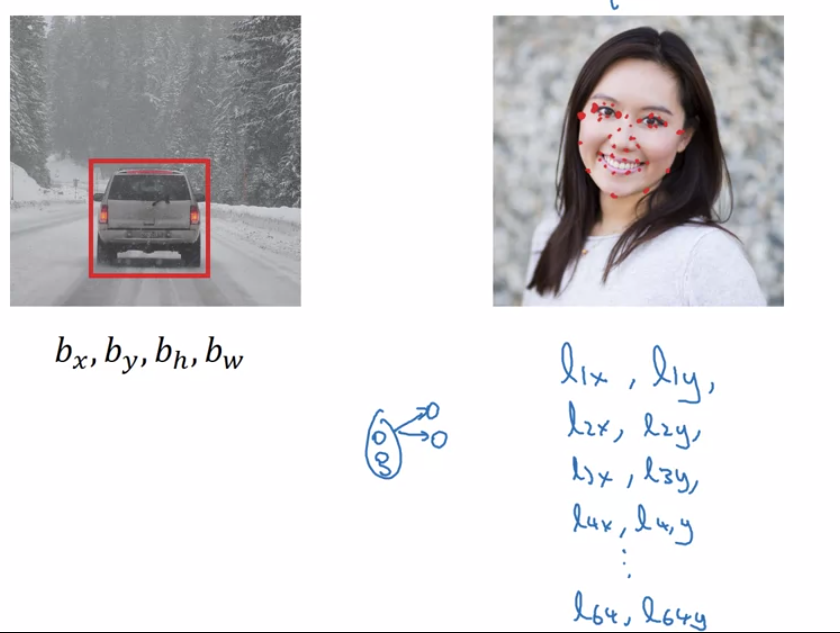
\includegraphics[scale=0.5]{Res/Lendmark_detection.png}
\caption{The difference between the bounding box and the landmarks.}
\label{Lendmark_detection.png}
\end{figure}

Now our network outputs if there's an image and a set of nodes for the $x$ and
$y$ position of each landmark.

When training, it's important to have consistent landmarks. That means we must
always have the same amount of lendmarks and they must be in the same location.
So if lendmark $1$ is the left corner of the left eye, that must be true for all
imagens.

\subsection{Slinding windows detection algorithm}%
\label{sub:slinding_windows_detection_algorithm}

Let's now see a basic algorithm for solving object detection algorithms.

So if we have images of cars and we have an algorithm that solves the problem of
classifying the image as a car or not car, then we can now take a picture with
many cars and slide a window across the image, checking if each window is or not
a car. If it is a car, then we have a bounding box (the window we are currently
in).

We might change the window size the slide for many sizes.

This concept is very similar to that concept of passing a convolutional filter
over a matrix.

Of course, the computational cost of this algorithm is very high, because each
time we slide the window, we have to ask the network is that new image is or not
a car (or any object we're detecting).

Fortunately, there's a much singler and cheaper way to implement this algorithm
using convolutions. To understand that, though, we have to understand how to
turn fully connected layers into convolutional layers. Let's see that first.

Suppose we have a $5\times 5\times 16$ volume and pass it to a $400$ node FC.
Then we could instead of that use $400$ filters of $5\times 5\times 16$. Then
the resulting dimention will be $1\times 1\times 400$. So instead of viewing
that FC layer as a plain stuff, we say it has a depth of $400$.

\begin{figure}[h]
\centering
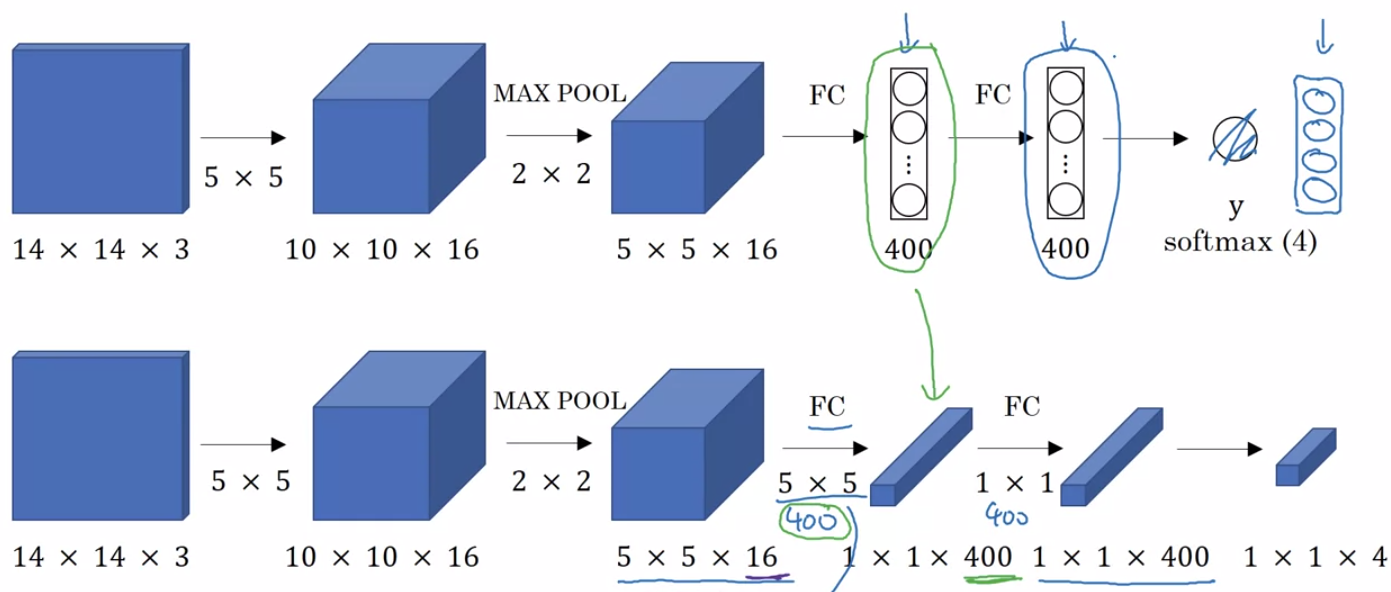
\includegraphics[scale=0.4]{Res/fc_into_conv_layers.png}
\caption{The difference between the FC layers and Conv layers.}
\label{fc_into_conv_layers.png}
\end{figure}

Now let's see how to speed up the sliding window algorithm.

So suppose we have a $16\times 16\times 3$ data set and the ConvNet of figure
above. In the original sliding window algorithm, we would apply the ConvNet four
times (stride of 2) in the images. But instead of that, what we do is just feed
the $16\times 16\times 3$ images into the ConvNet, resulting in a $2\times
2\times 4$ output. Each ``square`` on that output is equal to one window in the
original algorithm.

\begin{figure}[h]
\centering
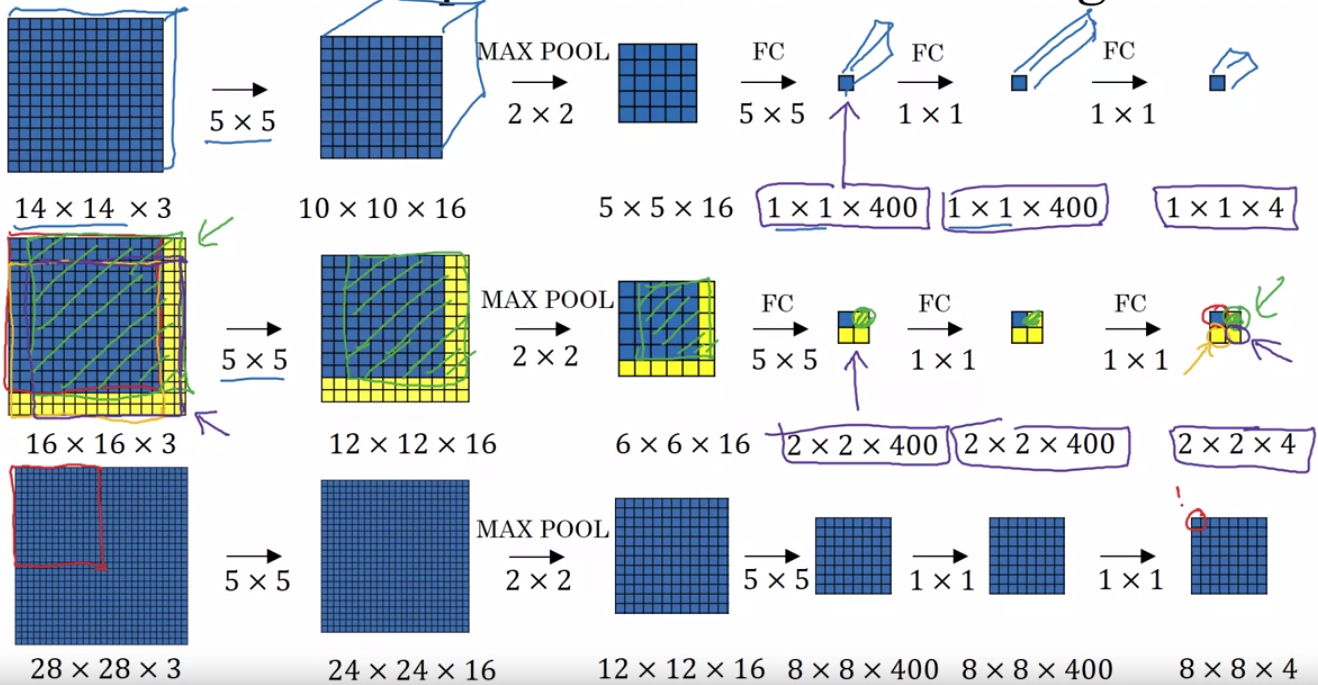
\includegraphics[scale=0.4]{Res/conv_sliding_windows.png}
\caption{Each square on the final output represent one window of the original
one, but everything is done with one pass.}
\label{conv_sliding_windows.png}
\end{figure}

\subsection{YOLO algorithm}%
\label{sub:yolo_algorithm}

Even using the convolutional aproach, the sliding windows algorithm will not
output precise bounding boxes, because it depends on the window size the stride
used. The YOLO algorithm, however can do that also with only one pass of a
convolutional network (what's why it's called \textit{You Only Look One}).

In this algorithm, you divide the original image into a grid ($3\times 3$ in the
example, but much bigger grid in real life). Now each square of the grid is
considered a single image and we apply the localization algorithm we've learned
later. Therefore, for each square we'll have a probability of containing an
object, a bounding box and a one-hot encoding. So let's suppose the one-hot
enconding contains $3$ numbers. Then we'll have a ``global'' output of $3\times
3\times 8$ ($1+4+3=8$).

What we do then is use a convolutional network with the size of the input that
maps to that $3\times 3\times 8$ output. The network will predict the whole
image at once, but will output at maximum one bounding box per square in the
grid, which is awesome.

\begin{figure}[h]
\centering
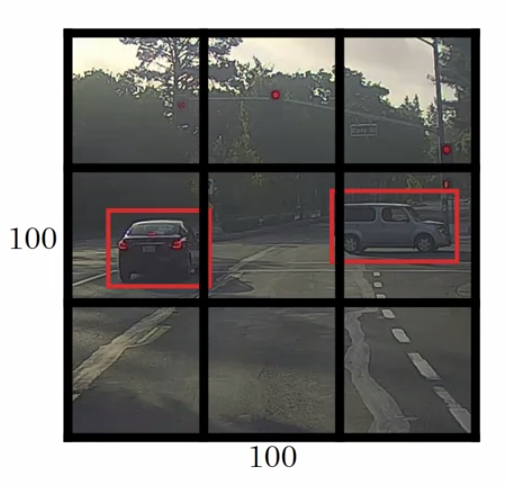
\includegraphics[scale=0.5]{Res/yolo_example.png}
\caption{Here we see an example of the grid in the YOLO algorithm.}
\label{yolo_example.png}
\end{figure}

We just need to note some things about this method.
\begin{enumerate}
    \item \textit{An object could be between two or more squares.} What we do
        then? In that case, we asign the object using its central point. The
        cell with the central point is considered the cell where that object is
        at;
    \item \textit{How to train the network? How to create the training
            examples?} To do that, we use the convention that the upper-left
            corner of the image is $\pair{0}{0}$ and the lower-right is
            $\pair{1}{1}$. Then $b_x$ and $b_y$ will be values between $0$ and
            $1$ and $b_h$ and $b_w$ represent the percentage of coverage of the
            image. In particular, they can be greater than $1$ when the bounding
            box is greater than a single cell.
\end{enumerate}

\subsubsection{Intersection over Union}%
\label{ssub:intersection_over_union}

To if an algorithm is predicting correctly a bounding box, we use the concept of
\textit{Intersection over Union} (or IoU). To compute that, we take the
predicted bounding box and the real bouding box and compute the intersection and
union of both, than we divide the union by the intersection. The closer to $1$,
the better. In particular, the value is $0$ is the intersection is null (the
predicted bounding box is completely out the real bouding box) and is $1$ if the
bouding boxes are exactly the same.

In general we use $0.5$ as a good value to achieve, but you might change that
acording to your needs.

\subsubsection{Non-max Suppresion}%
\label{ssub:non_max_suppresion}

In YOLO, we divide the image into many cells and an object might fall into many
of them and many of them might detect that same object. We need therefore a way
to keep just one bounding box for each object. How to do that with an algorithm?

What's where the \textit{non-max suppresion} comes into play.

In this algorithm, we select the bounding box with the highest $p_c$ and look at
all the remaining rectangles to check if any of them has a high IoU. If so, them
we remove those bounding boxes, because they belong to the same object (of
course, we look only at those that were predicted for the same object we're
looking right now). Them we do that again for the second highest $p_c$ and so
on, until we only have one bouding box for each object.

\begin{figure}[h]
\centering
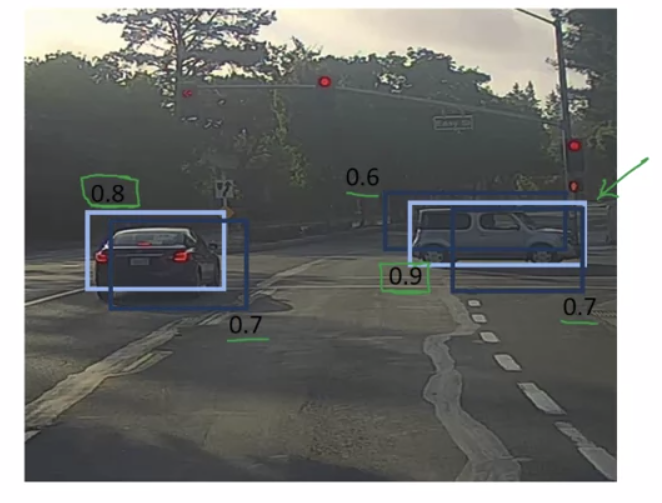
\includegraphics[scale=0.4]{Res/non_max_suppression_example.png}
\caption{Here we see an example of non-max suppresion. The bouding boxes with
$p_c$ equals to $0.9$ and $0.8$ are kept while the others will be excluded. Also
notice that we don't exclude the bb with $p_c=0.8$ when looking at the one with
$p_c=0.9$ because they have an IoU of $0$ and, thus, aren't the same object.}
\label{non_max_suppression_example.png}
\end{figure}

\subsubsection{Anchor Boxes}%
\label{ssub:anchor_boxes}

\textit{What if one cell of our grid wants to detect multiple objects?}

Let's suppose we have a car and a pedestrian in front of it and their center
points are so close together that fall into the same cell. That's one of the
reasons why to use \textit{anchor boxes}.

In this concept, we allow a cell to predict many bounding boxes according to a
predefined shape, called anchor box. In this case, we could predefine two anchor
boxes, one which is in a portrait shape and another in a landspace shape. the
portrait one will detect the car and the landspace one will detect the
pedestrian.

So now instead of having that $8$ nodes output for each cell of the grid (in our
previous example), we would have $16$ nodes for each cell, because we would have
two probabilities, two bounding boxes and two one-hot encodings.

\begin{figure}[h]
\centering
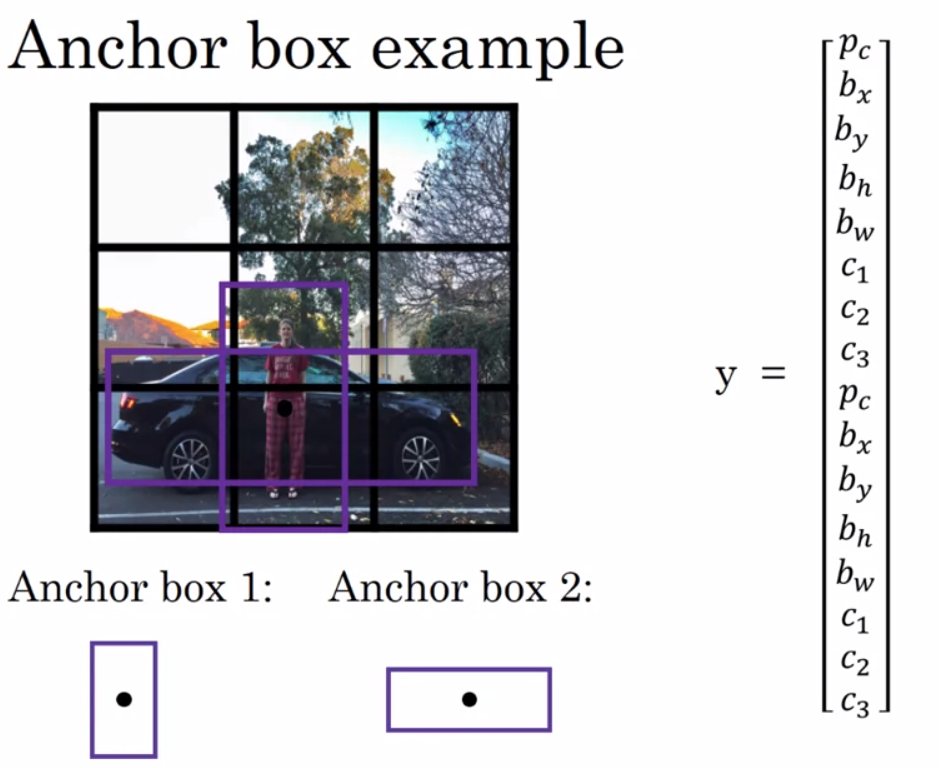
\includegraphics[scale=0.4]{Res/anchor_box_example.png}
\caption{Here we see the example showing the anchor boxes predefined and how the
$y$ label will look like for each cell of the grid.}
\label{anchor_box_example.png}
\end{figure}

One doubt might be how we should where we'll predict a class if we just have one
class. Well, in that scenario, we'll output it to the anchor box that is more
closer to the bounding box we're predicting. We use the IoU of the bounding box
with the anchor box and output to the anchor box that is closer to what we're
predicting.

If in the example the upper output ($p, b$ and $c$) refer to anchor box 1 and
the lower output refer to anchor box 2, then we're likely to predict pedestrians
using the lower part of the output and cars using the upper part.

One might think that this concept is very useless because that cenario where a
single cell wants to predict more than one bb is very unlikely to occour and the
downside of doubling the output is greater than that benefit. But actually if we
match the anchor boxes to the usual shape of the classes we want to predict,
than it can contribute to our algorithm because each output cell will be
specialized in predicting a certain class.

In our example, some cells will always predict the pedestrians and others will
always predict cars (because pedestrians have that portrait shape while cars
have a landspace one).

\section{Semantic Segmentation}%
\label{sec:semantic_segmentation}

In this section we're going to explore another vision problem: \textit{semantic
segmentation}.

In this kind of problem, instead of identifying objects using bounding boxes, we
input an imagem and want the network to color every single pixel with a color
that corespond to a particular kind of object. All the sky will be colored in
black, all the cars will be colored in brown, all the buildings will be colored
in blue and so on.

\begin{figure}[h]
\centering
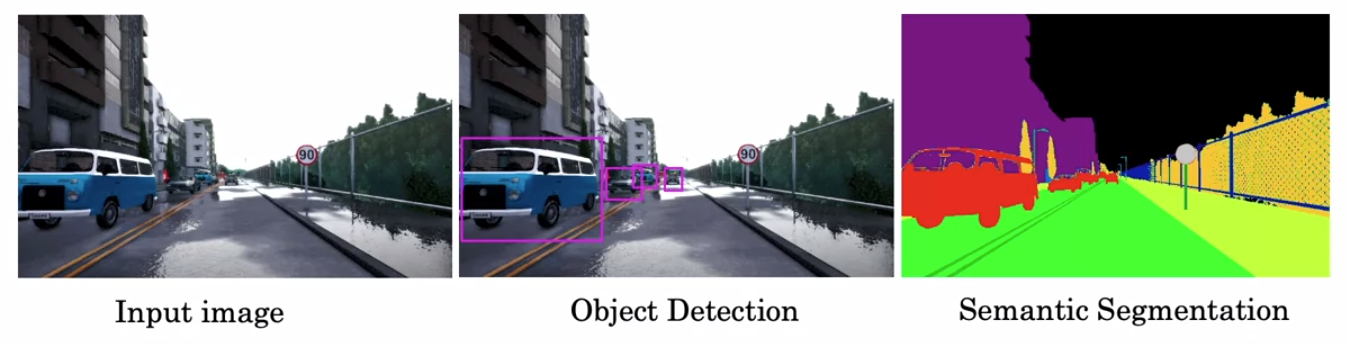
\includegraphics[scale=0.45]{Res/object_detection_vs_semantic_segmentation.png}
\caption{In the picture we see the differences between object detection and
semantic segmentation problems.}
\label{object_detection_vs_semantic_segmentation.png}
\end{figure}

So how to do that? The CNNs we've seen so far are only able to make the input
smaller and smaller (and deeper), but we need a away of applying convolutions
and after a while, making the shape of the computations go back to the original
size. To make that, we'll need to implement a \textit{transpose convolution}.

\begin{figure}[h]
\centering
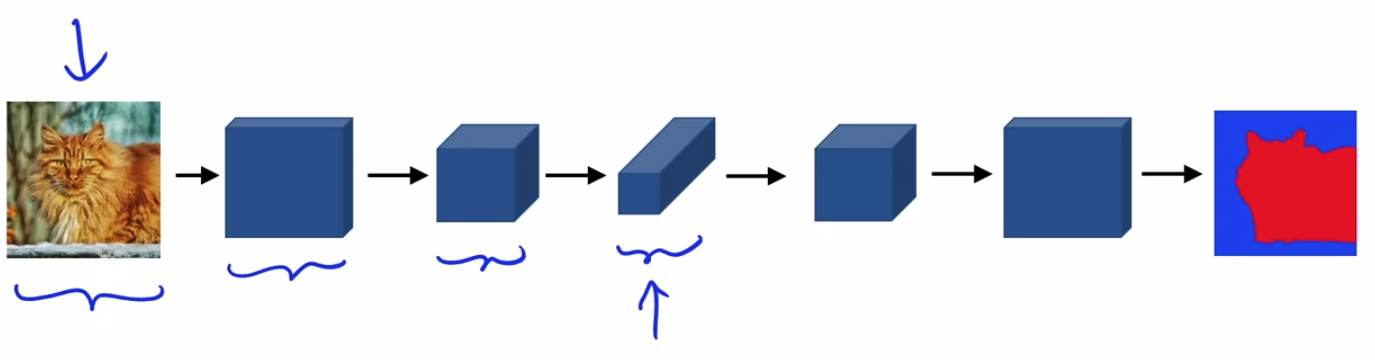
\includegraphics[scale=0.45]{Res/nn_for_semantic_segmentation.png}
\caption{Here we see an example of neural network for semantic segmental. We
decrease the height and weight and increase the number of channels until some
point and them increase the height and weight and decrease the number of
channels to the original size.}
\label{nn_for_semantic_segmentation.png}
\end{figure}

\subsection{Transpose Convolutions}%
\label{sub:transpose_convolutions}

Understanding transpose convolutions is very important to understand how to get
a $2\times 2$ input and blow it up to a $4\times 4$ output (or any input smaller
than output).

To learn that, let's use an example. Suppose we have a $2\times 2$ input and
want a $4\times 4$ output. So we're going to use a $3\times 3$ filter, padding
of $1$ and stride of $2$.

Our input and filter look like:

\[
I = \begin{bmatrix}
    2 & 1 \\ 3 & 2
\end{bmatrix}
\t\t
F = \begin{bmatrix}
    1 & 2 & 1 \\
    2 & 0 & 1 \\
    0 & 2 & 1
\end{bmatrix}
\]

First, we initialize the output matrix with zeros and pad it by $1$ (yes, we pad
the output, not the input).
Then, for each entry in the input, we're going to perform the following
operations:

\begin{enumerate}
    \item Multiply the filter matrix by that number;
    \item Now put the filter matrix in the right position in the output matrix
        (I'll show what I mean by right position in the figure);
    \item Then sum each element in the filter with the current element on the
        position that match with the filter entry.
\end{enumerate}

Simple like that!

Now what I mean by ``right position''? As we've padded the output matrix, now
it's $6\times 6$. So for the entry $0,0$ of the input matrix, I'll match the
$0,0$ entry of the filter with the $0,0$ entry of the output matrix.

\begin{figure}[h]
\centering
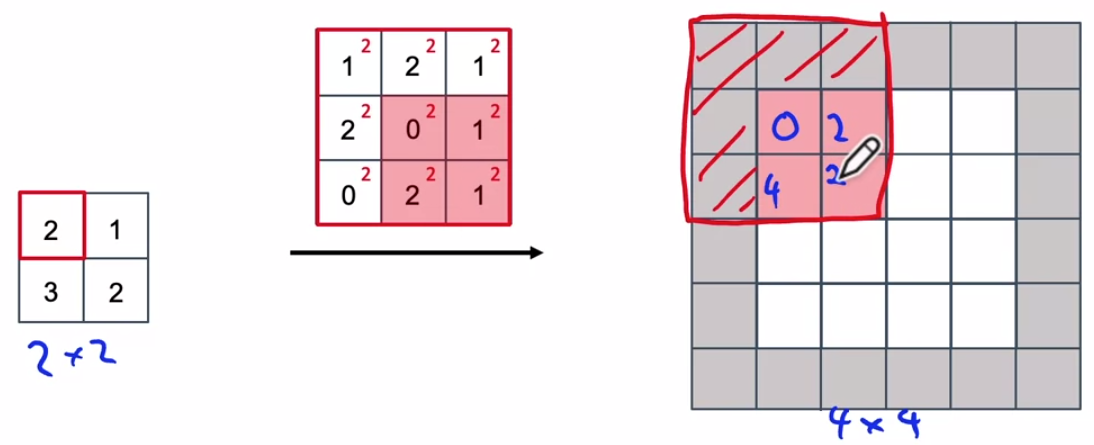
\includegraphics[scale=0.3]{Res/transpose_conv_1.png}
\caption{Here we see what happens in the first step of the transpose
convolution. We multiply the filter by $2$, put it in the $0,0$ position of the
output matrix and put the numbers on the right spots (ignoring the padding
because it will not enter in the final output).}
\label{transpose_conv_1.png}
\end{figure}

Then, I move on to the next entry in the input matrix, which is $0,1$. Since we
have a stride of $2$, will multiply those coordinates by $2$ resulting in $0,2$.
Now I put the filter in the $0,2$ entry of the output matrix and sum the filter
numbers as I said before.

Then, I move to $1,0$ and, therefore, match the filter if the position $2,0$ of
the output matrix.

\begin{figure}[h]
\centering
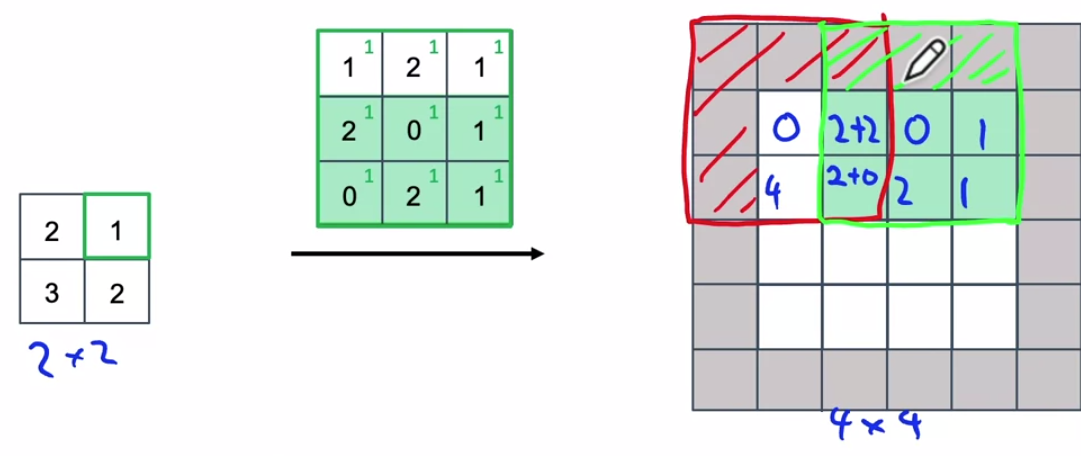
\includegraphics[scale=0.25]{Res/transpose_conv_2.png}
\caption{Here we see the next step of the covolution.}
\label{transpose_conv_1.png}
\end{figure}

\begin{figure}[h]
\centering
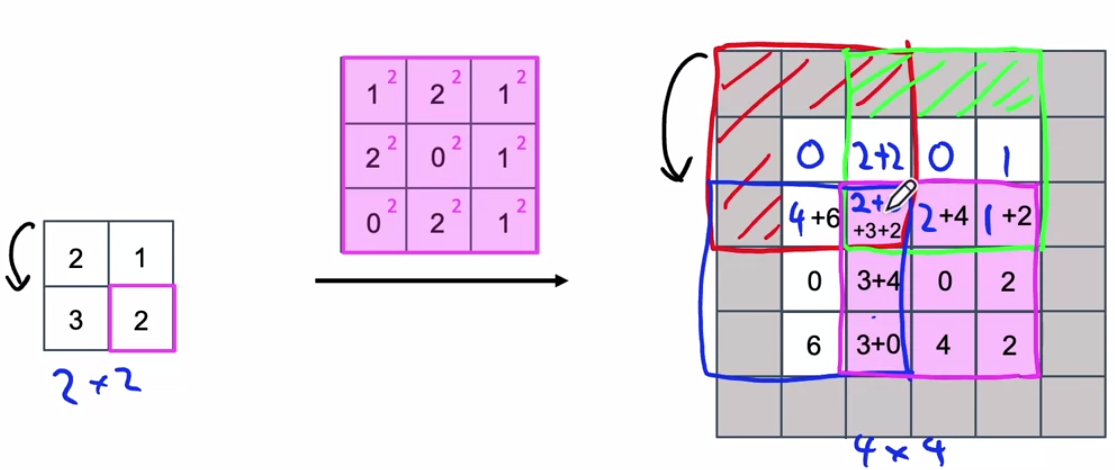
\includegraphics[scale=0.25]{Res/transpose_conv_3.png}
\caption{Here is the output matrix at the end of the transpose convolution.}
\label{transpose_conv_1.png}
\end{figure}

At the end, our output matrix will be:

\[
O = \begin{bmatrix}
    0 & 4 & 0 & 1 \\
    10 & 7 & 6 & 3 \\
    0 & 7 & 0 & 2 \\
    6 & 3 & 4 & 2
\end{bmatrix}
\]

\subsection{U-Net}%
\label{sub:u_net}

Now we'll use the transpose convolutions to build a U-Net, which is the main
architecture for solving semantic segmentation problems.

So as we've seem before, we use normal convolutions to reduce the image into a
smaller shape and then we use transpose convolutions to make it back to the
original shape. That small shape region will help us to reduce the amount of
information about the image, forcing the network to really learn the fundamental
of that we're trying to map.

But also, there's one more stuff we need to add to that architecture to call it
a U-Net, and that's skip connections from the normal convolution part to the
transpose convolution part. Those skip connections will make the model use not
just the fundamental information of the image, but also join that with the
high resolution information contained in the first half of the network.

Let's take a look at the U-Net architecture.

\begin{figure}[h]
\centering
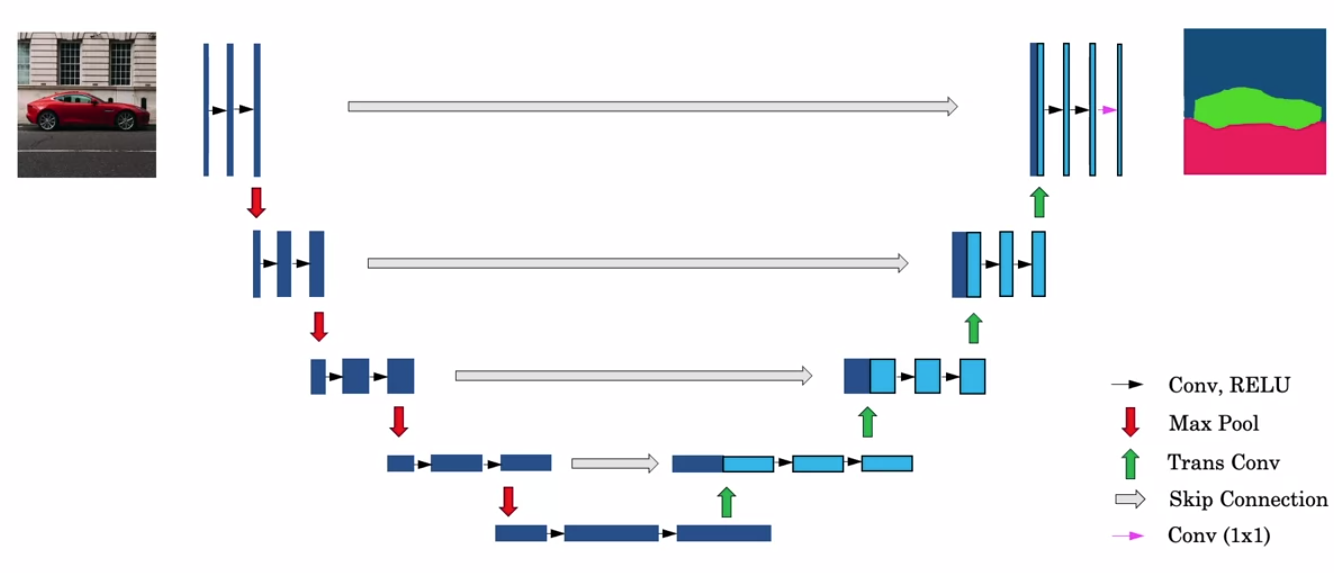
\includegraphics[scale=0.45]{Res/u-net_architecture.png}
\caption{That's the original U-Net architecture.}
\label{u-net_architecture.png}
\end{figure}

We can see that in this architecture, we use convolutions actually with the
``same'' padding, to keep the input size and than use a max pooling layer to
reduce the input size. Each time we use two conv layers and one max pooling
layer.

Than, after a while, we start using transpose convolution layers instead of max
pooling, to return to the original size. So we do two conv layers and one trans
conv layer (but in the first conv layer we have a skip connection from the part
of the network where we had the same size, but in the first half).

At the end, we have a $1\times 1$ convolution to get our output.

One can see that the architecture is called U-Net becuase it looks like an U. We
have a \textit{downscaling part}, a \textit{bridge part} and a \textit{upscaling
part}.

\section{Face Recognition}%
\label{sec:face_recognition}

Before moving to the face recognition problem, we have to talk about the
\textbf{face verification} problem, in which we're given an input image and a
name/ID and need to output whether the input image is that of the claimed
person. That's called a one to one problem.

The recognition problem is much harder, because it envolves more than one
person. In the face recognition problem, we have a datebase with $K$ persons
and, given an input image, we need to ouput the ID of the person if the image is
any of the $K$ persons in the database or output ``not recognized''. That a one
to $K$ problem.

If we have a face verificiation system with a $99\%$ accuracy and apply it to
the recognition problem, we'll have $K$ times more chances of having an error,
because now we have $K$ persons.

\subsection{One-shot learning}%
\label{sub:one_shot_learning}

One-shot learning is a kind of machine learning algorithm that just need one
input to be trained. In the case of a face recognition problem, that's quite
often because we might have just one photo of each person in our database and
want to, given a new photo, predict if it's from anyone in the database or is
not present in the database.

We could apply the image into a CNN and predict a vector of $k+1$ dimention with
a softmax layer where $k$ is the number of persons. That vector is the
probability of each person or none of them (that why the $+1$). That however is
very unlikely to give good results because just one photo isn't enough to train
a CNN. The what if we want to add new people to the datebase, we would need to
retrain the CNN, losing everything.

In this kind of problem, we want to learn a ``similarity'' function, which is a
function $d(img1, img2)$ measuring the degree of difference between images.

Is that degree is low for two images (below a threshold $\tau$), we say the two
images belong to the same person.

\subsection{Siamese network}%
\label{sub:siamese_network}

But how to actually learn that $d$ function? One good way is using a
\textit{simamese network}. In this kind of neural network, we have a simple CNN
just like we had throughout this chapter, with some Conv Layers and some FC
Layers at the end. But just in the head (the last layer) of that network,
instead of having a softmax unit to output some small vector, we actually cut
that and have a big FC layer at the end. Let's suppose we have a FC layer with
say $128$ units.

We define this output as an \textit{encoding} of the input. So if we apply a
picture $\xii[x]{1}$ through the network, it will output the encoding of that
image $f(\xii[x]{1})$.

Therefore, each image $\xii[x]{i}$ has an encoding $f(\xii[x]{i})$. What we want
now is to compare those encodings in a way that the same person will have
similar encodings.

So we can use $d(\xii[x]{i}, \xii[x]{j})$ as $\norm{\xii[x]{i}-\xii[x]{j}}^2$.
And we want $d$ to be a large number if $i$ and $j$ are different people and $d$
to be a small number if they're the same. We need, then, to make our network
learn parameters such that these conditions are satisfied using backpropagation.

\subsection{Triplet Loss Function}%
\label{sub:triplet_loss_function}

To train a siamese network, we need to define a loss function. The main loss
function used is the \textit{triplet loss function}, which needs two photos of
the same person and one photo of another person.

For this loss function, we set an \textit{anchor}, a \textit{positive} instance
and a \textit{negative} instance. That's our triplet $\angbracket{A, P, N}$.

What we want now is to set the difference between the anchor and the positive case
to be lower than the difference between the anchor and the negativa case. That
leads to the equation:

\[
\norm{f(A)-f(P)}^2 \leq \norm{f(A)-f(N)}^2
\]

However one might see that it can be solved quite trivialy by just predicting
zeros or actually by predicting the same value for any image. If $f(x) = c$ for
a constant vector $c$, then we would have $0\leq 0$ always, which would be
interpreted as a good thing.

That's why we also add a \textit{margin term} $\alpha$, which is a
hyperparameter. We say that the difference between those differences much be at
least $\alpha$. In the equation
we have:

\[
\norm{f(A)-f(P)}^2 + \alpha \leq \norm{f(A)-f(N)}^2
\]

or:

\[ \boxed{
\norm{f(A)-f(P)}^2 - \norm{f(A)-f(N)}^2 + \alpha \leq 0
}\]

And now we define the error function as a sum over all the triplets:
\[
\mathcal{L}(A, P, N) = \max\paren{
    \norm{f(A)-f(P)}^2 - \norm{f(A)-f(N)}^2 + \alpha, \,0
}
\]
\[ \boxed{
J=\sum_{i=1}^{n} \mathcal{L}\paren{\xii[A]{i}, \xii[P]{i}, \xii[N]{i}}
}\]

Also, one might see that we need more than one picture per person to train the
network. Our training set could have $10$k picture of $1$k people, with an
average of $10$ pictures per person.

When training the network, we do need more than one photo, but when applying it
just to encode a new person, we'll not need more than one photo because we are
assuming our network learned how to encode a photo in a way that's good to, when
exposed to a photo of the same person, have a close encode.

\jump

Now the question we still need to answer is how to choose our triplet
$\angbracket{A, P, N}$. If we choose very different people, our constrain will
be easily satisfied, so we need to, somehow, this to make is hard for the
network (show hard examples).

And we actually know what's hard for the network because, when training, some
triplets will have $d(A, P)$ and $d(A, N)$ much closer than others. These are
the ones we like, because they will push the network futher into increasing
$d(A, N)$ or decreasing $d(A, P)$ until the point the difference is smaller than
$\alpha$.

Therefore, we chose the triplets there aren't still satisfied.

\subsection{Face Verification as a Binary Classification Problem}%
\label{sub:face_verification_as_a_binary_classification_problem}

Instead of using the Triplet Loss Function that we've seem before, we can also
concatenate the outputs of the simamese network into a final logistic regression
output that predictes $1$ is the images are the same person or $0$ if it's not.

That's a nice way of learning a similarity function instead of creating one.

\begin{figure}[h]
\centering
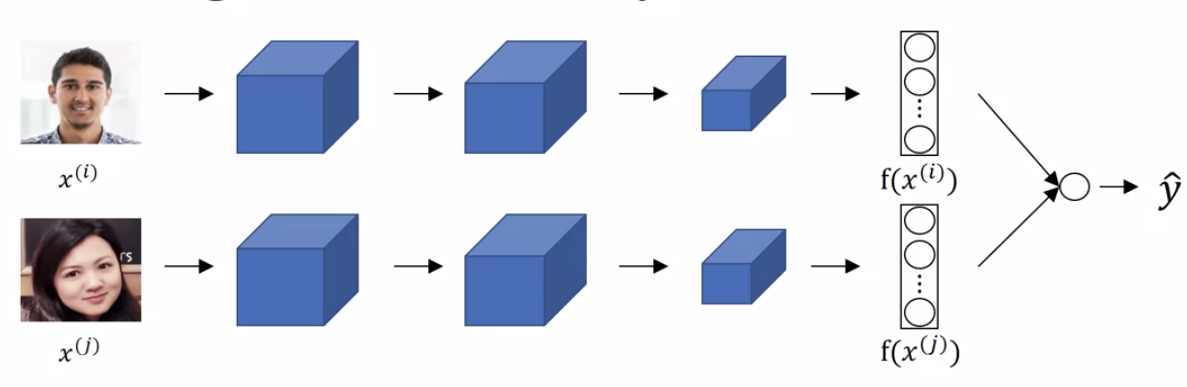
\includegraphics[scale=0.5]{Res/simamese_binary_class.png}
\caption{We pass both images through the same CNN, which encodes them into a
feature vector and use those vectors as inputs for a final layer which predicts
$1$ or $0$. If we're not in the training fase, but in the deploy face of our
project, we can precompute the encodings of the saved people the use the input
to compare with all of them and check if the input is any of the saved people.}
\label{simamese_binary_class.png}
\end{figure}

\section{Neural Style Transfer}

\textbf{Neural Style Transfer} is a technique that allow us get any image and
apply a style of another image over it.

\begin{figure}[h]
\centering
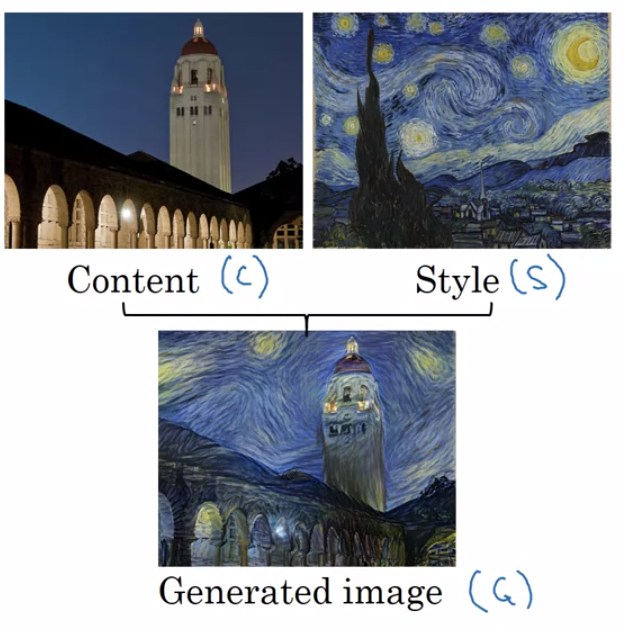
\includegraphics[scale=0.5]{Res/neural_style_transfer.png}
\caption{Here we have an example of neural style transfer.}
\label{neural_style_transfer.png}
\end{figure}

In order to transfer a style, we need to get all the features learned in many
different layers of a ConvNet. So let's understand a little better what exactly
is a CNN learning.

To get intuition on that, let's make an exercise of picking a single neuron unit
in a layer of the network. Then let's plot all the images that maximize the
activation of that unit. But since a neuron in the first layer don't actually
sees much of the image, we're going to plot only the pixels that the neuron
really sees in that image of maximum activation.

\begin{figure}[h]
\centering
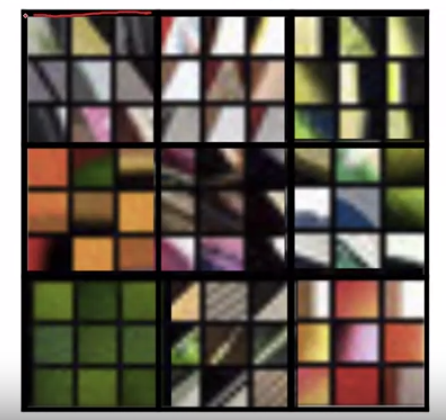
\includegraphics[scale=0.5]{Res/visualizing_cnn_1.png}
\caption{This figure shows the $9$ images for $9$ random nodes in the first
layer of a CNN. These images are the ones that maximize the respective neurons.
We can clearly see that each $3\times 3$ square in the matrix above detects a
different pattern of image. Most of them detect lines with some particular
colors. That's because in we got neurons from the first layer.}
\label{visualizing_cnn_1.png}
\end{figure}

Plotting that that, we'll get a figure like \ref{visualizing_cnn_1.png}. Let's
now repeat that for other layers.

\begin{figure}[h]
\centering
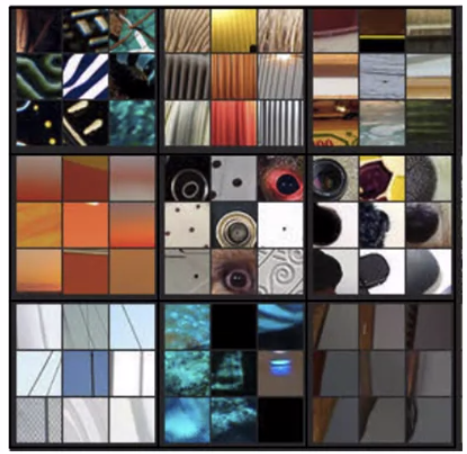
\includegraphics[scale=0.5]{Res/visualizing_cnn_2.png}
\caption{This figure shows the same as the previous, but for neurons from the
second layer. We see that we're building complexibility.}
\label{visualizing_cnn_2.png}
\end{figure}

\begin{figure}[h]
\centering
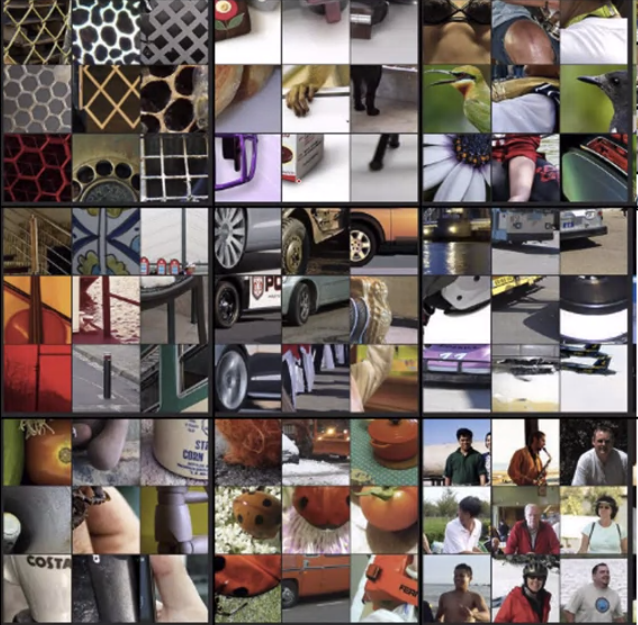
\includegraphics[scale=0.5]{Res/visualizing_cnn_3.png}
\caption{Now we see the same as the two previous figures, but for layer 3. We
can see that a neuron is detecting people, while other is detecting tires and so
on. We observe that each neuron is learning a different complex pattern.}
\label{visualizing_cnn_3.png}
\end{figure}

\subsection{Cost Function}%
\label{sub:cost_function}

The first step to apply neural style transfer is creating a cost function. So
let's remember that we have a Concent $C$, a Style $S$, and want a Generated
image $G$. We want to define $J(G)$ to be the cost function. Then, we can use
Gradient Descent to minimize that function.

We'll break that cost function into two parts, the concent cost and the style
cost:

\[
J(G)=\alpha J_{\text{content}}(C, G) + \beta J_{\text{style}}(S, G)
\]

The style cost measures how close is the style of S to the style of G, and the
content cost measures how close is the content of C to the content of G. We'll
average those costs using two hyperparameters $\alpha$ and $\beta$.

We could really just use one hyperparameter, but the original authors of the
technique use two, so we'll just do the same.

After defining the cost function, we initialize $G$ randonly and run gradient
descent updating the pixels of $G$ until it looks good.

\paragraph{Content Cost Function}%
\label{par:content_cost_function}

For the content cost function, we recall on what we've seen before on what each
layer of the ConvNet learns. To define this cost, we get a pre-trained CNN and
select a layer $l$ (nether too shallow or too deep). If we run two images, that
layer will have different outputs. Those outputs can be similar or not, but in
general they will be similar if the \textit{content} of both images is similar.
So we'll define that difference as the content cost function.

Formally, if we have two images $C$ and $G$, let $\xlayer[\xii[a]{l}]{C}$ and
$\xlayer[\xii[a]{l}]{G}$ be the activations of layer $l$ on those images. Then,
we define:

\[
J_{\text{content}}(C, G)=\dfrac{1}{2}
\norm{\xlayer[\xii[a]{l}]{C}-\xlayer[\xii[a]{l}]{G}}^2
\]
\begin{obs}
We're using $a$ as a flattened vector of the layer.
\end{obs}

\paragraph{Style Cost Function}%
\label{par:style_cost_function}

To measure the style of an image, we need to define what is style.

Formally, we'll define it as the \textit{correlation between activations across
different channels of a convolutional layer}. Let's understand what that mean.

Basicaly we've seen before that each activation (neuron) detects different kinds
of shapes and patterns in an image. We can define the style as the correlation
of those patterns (i.e., if a pattern is present in an image, than another
pattern is also present). This gives us a formal way to express style.

So to calculate that, we need to define a \textit{style matrix} $G$.

First, let's define $\xlayer[a]{l}_{i,j,k}$ as the activation at $(i,j,k)$ of
our convolutional layer. The matrix $\xlayer[G]{l}$ is
$\xlayer[n]{l}_c\times\xlayer[n]{l}_c$ (a squared matrix of dimensions equal to
the number of channels of a layer). An element $\xlayer[G]{l}_{k,k'}$ of the
matrix computes the correlation for layer $l$ between channel $k$ and $k'$.

To compute the matrix, we compute each element as:

\[
\xlayer[G]{l}_{k,k'}=\spsum{i=1}{\xlayer[n]{l}_H}\spsum{j=1}{\xlayer[n]{l}_W}
\xlayer[a]{l}_{ijk} \xlayer[a]{l}_{ijk'}
\]

\begin{obs}
The right formula actually indicate that those values are calculated over the
Style $S$, but I'll ommit that since the formula would be too populated.
\end{obs}

We now define the style cost function for a particular layer $l$ as:

\[
\xlayer[J]{l}_{\text{style}}(S,G)=
\dfrac{1}{\paren{2\xlayer[n]{l}_H\xlayer[n]{l}_W\xlayer[n]{l}_C}^2}
\norm{\xlayer[\xii[G]{l}]{S}-\xlayer[\xii[G]{l}]{G}}^2
\]

or

\[ \boxed{
\xlayer[J]{l}_{\text{style}}(S,G)=
\dfrac{1}{\paren{2\xlayer[n]{l}_H\xlayer[n]{l}_W\xlayer[n]{l}_C}^2}
\spsum{k}{}\spsum{k'}{}
\paren{G_{kk'}^{[l](S)}-G_{kk'}^{[l](G)}}^2
}\]

And the authors found out that the result is better if we sun those correlations
between many different layers, so the final style cost function is:

\[ \boxed{
    J_{\text{style}}=\spsum{l}{}\lambda_l \xlayer[J_{\text{style}}]{l}(S,G)
}\]

and we use an additional set of hyperparameters $\lambda_l$ for that.

Finally, the final cost function will be:
\[ \boxed{
J(G) = \alpha J_{\text{content}}(C, G) + \beta J_{\text{style}}(S, G)
}\]

%%%%%%%%%%%%%%%%%%%%%%%%%%%%%%%%%%%%%%%%%%%%%%%%%%%%%%%%%%%%%%%%%%%%%%%%%%%%%%%%

\chapter{Sequence Models and Applications}%
\label{cha:sequence_models_and_applications}

Sequence problems are supervised problems where eather the input or the output
(or both) are sequences.

For a particular sequence input $x$, we'll denote the elements of the sequence
as $\xseq[x]{1}, \xseq[x]{2}, \cdots \xseq[x]{t}, \cdots \xseq[x]{T_x}$, where
$T_x$ denotes the lenght of the sequence. The same holds for $y$.

As we denote the $i$-th input as $\xii[x]{i}$, it means that the $t$-th element
of the $i$-th input is $\xii[\xseq[x]{i}]{t}$, and the length of the $i$-th
input is $\xii[T_x]{i}$. Again, the same holds for $y$.

\begin{figure}[h]
\centering
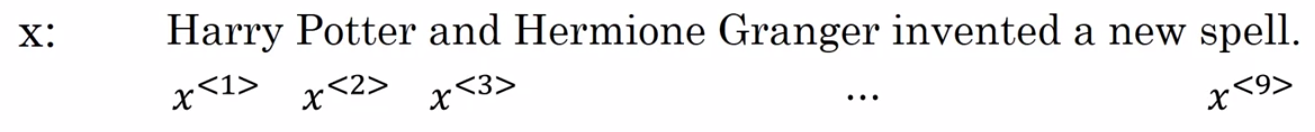
\includegraphics[scale=0.4]{Res/phrase_representation.png}
\caption{An example of phrase representation.}
\label{phrase_representation.png}
\end{figure}

\section{Recurrent Neural Network}%
\label{sec:recurrent_neural_network}

Now that we're familirized with the notation and the problem, let's see how to
create a model to learn and solve sequence problems.

The first step is understand why a simple NN doesn't work here.

So suppose we want to use the standard MLP model. So we feed the input sequence
and pass through some hidden layers and the output layer is also a sequence.
Seems like we could do that and indeed we can. But there are two main problems
with that aproach.

The first one is that the input and output sequences might have variable length.
If we're dealing with phrases, for instance, each phrase can have a difference
size.

But the bigger problem is that this aproach doesn't share features learned
across different positions of the sequence. Suppose we want to find all the
names in a phrase (like the one from Figure \ref{phrase_representation.png}).
The first node from the first layer might learned that \textit{Harry} is a name.
But as that node just get information from the first word of the text, it will
not spread that information that \textit{Harry} is a name to the other nodes
and, therefore, if \textit{Harry} apears in other parts of the text, we'll have
to learn that again and again for each position.

Also, as we've seen in the image part of the specialization, creating a mode
just for this kind of problem will help to reduce the number of features we have
to learn.

A Recurrent Neural Network (RNN) can help with the problem. In this kind of
architecture, we feed the input in different timestamps. At each time, the
network will compute an output and use its activation values (or some of them)
as inputs for the next timestamp.

\begin{figure}[h]
\centering
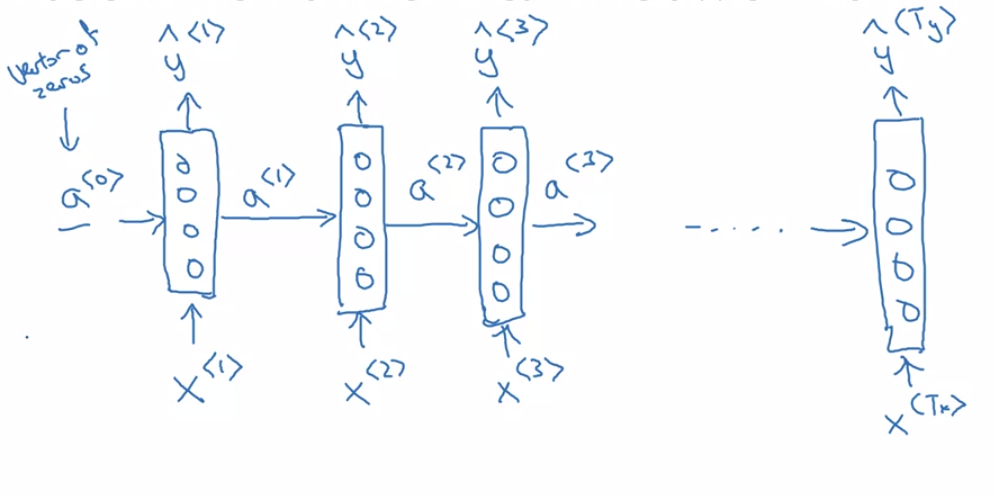
\includegraphics[scale=0.45]{Res/RNN_basic.png}
\caption{For the first element, we use only its value and an arbitrarial
$\xseq[a]{0}$ vector to compute $\xseq[y]{1}$. For the next element, we use both the
element and the activation $\xseq[a]{1}$ from the previous input.}
\label{RNN_basic.png}
\end{figure}

\begin{figure}[h]
\centering
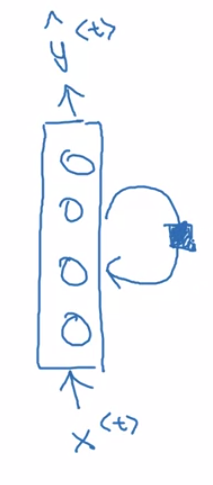
\includegraphics[scale=0.5]{Res/RNN_representation.png}
\caption{Some authors use this diagram to represent RNNs, the loop with a box
represents a delay of one timestamp.}
\label{RNN_representation.png}
\end{figure}

RNNs scan the input sequence from left to right and use the same parameters
for each element.

Scanning from left to right not always is a good thing. Many times we also need
information that we'll see on the right to predict something about the left
element. That's one limitation of this particular architecture. Later we'll see
how to address that.

To compute forward propagation, we use:
\[
\xseq[a]{t}=g\paren{W_{aa}\xseq[a]{t-1}+W_{ax}\xseq[x]{t}+b_{a}}
\]
\[
\xseq[y]{t}=g\paren{W_{y}\xseq[y]{t}+b_{y}}
\]

And to simplify the notation, we'll write the first formulata as:
\[
\xseq[a]{t}=g\paren{W_{a}\sbracket{\xseq[a]{t-1}, \xseq[x]{t}}+b_{a}}
\]

$W_a$ is the matrix that we get when stack horizontally $W_{aa}$ and $W_{ax}$
and $\sbracket{\xseq[a]{t-1}, \xseq[x]{t}}$ denotes the vector we get when
stacking vertically $\xseq[a]{t-1}$ and $\xseq[x]{t}$.

\subsection{Different types of RNNs}%
\label{sub:different_types_of_rnns}

So far, we only saw the type of RNN were the number of inputs and outputs is the
same. Let's explore some other types of more interesting RNNs.

The kind of architecture we've seen is called \textbf{many-to-many}, because we
have $T_x=T_y$ and they're both grater than one.

Another kind of architecture is called \textbf{many-to-one}, where we have a
sequence as input and a single output at the end of the architecture, after
we've read the whole sequence (or instance, sentiment classification of a
sentense).

We could also have a perhaps not very interesting architecture where
$T_x=T_y=1$. That's called \textbf{one-to-one}.

\begin{figure}[h]
\centering
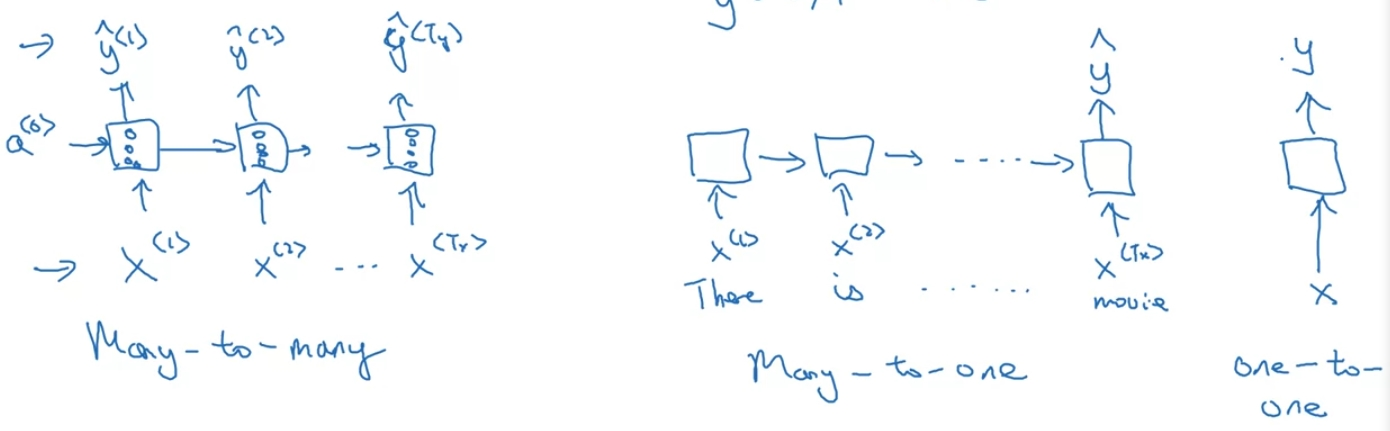
\includegraphics[scale=0.4]{Res/RNN-types.jpg}
\caption{Three different types of RNNs.}
\label{RNN-types.jpg}
\end{figure}

We may also have a \textbf{one-to-many} architecture that has a single input and
outputs a sequence. For instance, we may input a single note and want the NN to
create a song starting which that note. The input could also be null in that
case, but we still call that one-to-many.

To create that kind of architecture, we have the input be feeded in the first
pass through the neural network and before that, the input will be actual the
output of the last time we run the NN. So we use $x$ to predict $\xseq[y]{1}$
and then we use $\xseq[y]{1}$ as the input for the next time.

In the \textbf{many-to-many} case, there's no reason to have $T_x=T_y$, the
input and output might have different lenghts. To generate that kind of result,
we first feed all the $x$ values and get no output from the neural network.
Then, after feed them all, the neural network starts predicting the $y$ values
one by one.

The parts that receive the inputs and predict the outputs are actually different
and we call them the \textit{encoder} and \textit{decoder} respectively.

\begin{figure}[h]
\centering
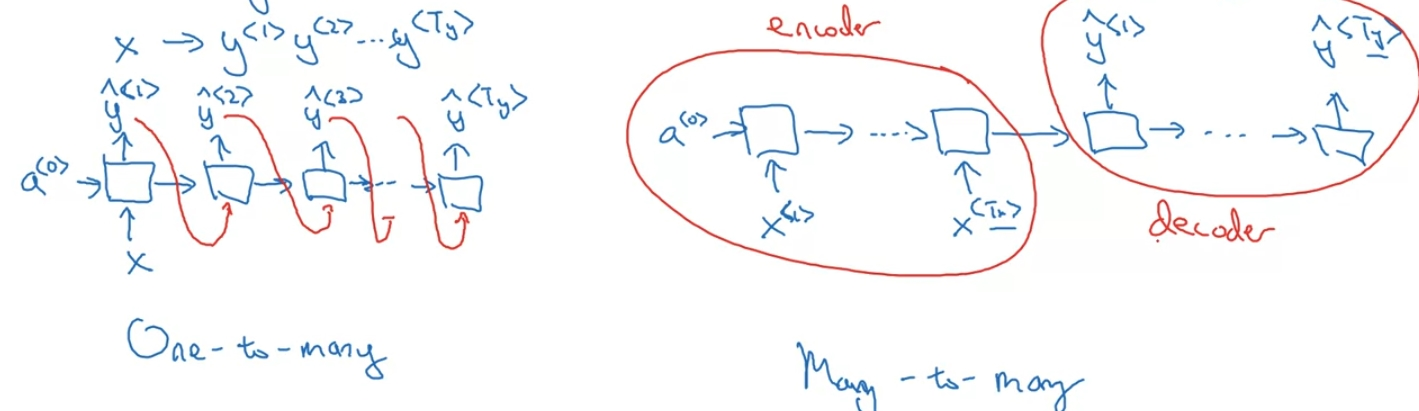
\includegraphics[scale=0.4]{Res/RNN-types2.jpg}
\caption{More examples of RNNs.}
\label{RNN-types2.jpg}
\end{figure}

\section{Language model and sequence generation}%
\label{sec:language_model_and_sequence_generation}

A language model is a function that, given any sentence, returns a probability
of that sentence.

Suppose we have a speech recognition system that is trying to guess if the
speacher said: \texttt{The apple and pair salad was delicious.} or \texttt{The
apple and pear salad was\nl delicious.}

As a human we know the second sentence is much more likely to be the correct
one. That the behavior that a language model tries to replicate.

To build such a model, we need a large corpus of english text. Than we need to
tokenize the sentences and use encodings to represent each word (we could use
one-hot encodings, for instance, but we'll see in the future that there are many
better ways to encode a word). Also, it's very common to add an extra token to
denote the end of sentence, written as \texttt{<EOS>}.

Other common special token we see is the \texttt{<UNK>} token, which denotes an
unknown word. If you have a vocabulary of say the $10.000$ most common english
words, then a egyptian name could not have a encoding representation, so we
simply encode it as \texttt{<UNK>}.

To train the langague model using an RNN, we we'll input it with many sentences
and, at each word, we'll try to predict the next word of the sentence. So in the
first step, we input the NN with $\xseq[x]{1}=\vec{0}$, because there's no
previous word. Than it will predict $\xseq[\hat{y}]{1}$, what it believe it's
the first word of the sentance.

Before that, we'll actually feed the NN with $\xseq[x]{2}=\xseq[y]{1}$. And
notice that it's not $\xseq[\hat{y}]{1}$, but $\xseq[y]{1}$, the real first word
of the sentence. So now, with the first real word of the sentence, we try to the
predict the second word. And them we feed it with the next word $\xseq[y]{2}$
and so on until the end of the sentence.

\begin{figure}[h]
\centering
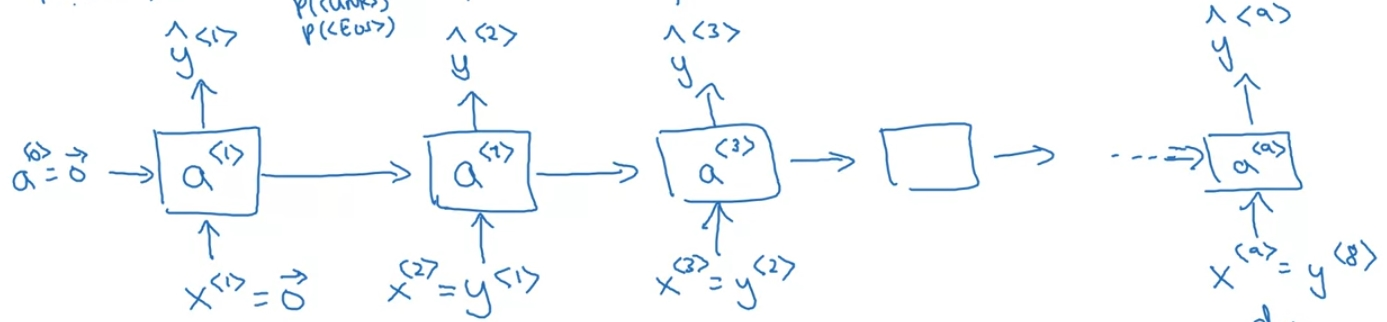
\includegraphics[scale=0.4]{Res/RNN-language-model.jpg}
\caption{An example of training an RNN to create a language model.}
\label{RNN-language-model.jpg}
\end{figure}

At the end, we compare each output word with the real output we excepted using
the cross entropy loss:
\[
\mathcal{L}(\xseq[\hat{y}]{t}, \xseq[y]{t}) =
-\spsum{i}{}\xseq[y_i]{t}\log \xseq[\hat{y}_i]{t}
\]

\subsection{Sampling Novel Sequences}%
\label{sub:sampling_novel_sequences}

After training a language model, we might want to have a view of what is it
predicting. To do that, we can use samples of sequences generated by the model.

To do that, we input $\xseq[x]{1}$ as $\vec{0}$, as we always do, and predict
$\xseq[\hat{y}]{1}$, which is a vector of probabilities for all the words in our
vocabulary. Now, instead of picking the word with highest probability, we'll
sample using that probability distribution (meaning that words with higher
probability have higher chances of beeing chose, but it's not deterministic).
After picking that word using the distribution, we feed it into the network
again in the next time stamp and repeat the process until a stop point.

That stop point can eather be a number of iterations or a condition, like if
\texttt{<EOS>} was picked, or if the probability of picking \texttt{<EOS>} is
larger than a threshold.

That process will generate many different sample santances that will tell us how
our model behavies.

\section{Vanishing gradients with RNNs}%
\label{sec:vanishing_gradients_with_rnns}

As we've already seen in other types of NNs, vanishign gradients is a common
problem. RNNs are also affected by that problem. Let's see how that problem is
handled with RNNs.

In sequence models, like language modeling, we can have term dependencies with
terms that are far apart, like in the examples: \jump

\texttt{The \textbf{girl} I met yesterday at the nightclub \textbf{was} pretty.}

\texttt{The \textbf{girls} I met yesterday at the nightclub \textbf{were} pretty.}
\jump

The RNN tends to ``forget'' about the terms it was a long time ago and,
therefore, it might be difficult to predict if we want the word \textit{was} or
\textit{were}. That's exactly the problem vanishign gradients cause.

In other NN architectures, we solved this problem using skip connections. But
here, we would need a skip connection \textit{through time}. \jump

The next sections will discuss some methods to adress this problem.

\subsection{Gated Recurrent Unit (GRU)}%
\label{sub:gated_recurrent_unit_gru_}

The GRU is a modification to the RNN neurons that make it much batter to capture
long term dependencies and solve the vanishing gradient problem.

That unit has a new variable called $c$ of \textit{memory cell}. At time $t$,
the memory cell will have a value $\xseq[c]{t}=\xseq[a]{t}$ (for the GRU $c$ is
equal to the activation value at that moment, but that will change for LSTM).

At each time, we'll have a candidate to replace $c$, which is:
\[
\xseq[\tilde{c}]{t}=\tanh\paren{W_{c}\sbracket{\xseq[c]{t-1},\xseq[x]{t}}+b_c}
\]

And we have a gate $\Gamma_u$:
\[
\Gamma_u=\sigma\paren{W_{c}\sbracket{\xseq[c]{t-1},\xseq[x]{t}}+b_c}
\]

And we update the memory cell using the gate and the candidate like so:
\[
\xseq[c]{t}=\Gamma_u\times\xseq[\tilde{c}]{t}+(1-\Gamma_u)\times\xseq[c]{t-1}
\]

\begin{obs}
Remember that $\sigma(x)$ is the sigmoid function, which can be thought as a
function that maps to either $0$ or $1$. Therefore, the formula above than be
though as keeping the old value if the gate is zero or updating to the candidate
if the gate is one.
\end{obs}

\paragraph{Full GRU}%
\label{par:full_gru}

There's another version of GRU, which is more commonly used. This version adds a
new parameters $W_r$, which is used to compute a new gate $\Gamma_r$ used to
check how relevante $\xseq[c]{t-1}$ is to calculate $\xseq[\tilde{c}]{t}$:

\[
\Gamma_r=\sigma(W_r\sbracket{\xseq[c]{t-1},\xseq[x]{t}}+b_r)
\]
\[
\xseq[\tilde{c}]{t}=\tanh\paren{W_{c}\sbracket{\Gamma_r\times\xseq[c]{t-1},\xseq[x]{t}}+b_c}
\]

All other equations are kept the same.

\subsection{Long Short Term Memory}%
\label{sub:long_short_term_memory}

The LSTM is a more powerful and general version of the GRU. This kind of cell
doesn't always have $\xseq[c]{t}=\xseq[a]{t}$. And also we don't have just one
gate for the update. We'll use an \textit{update} gate, a \textit{forget} gate,
and also an \textit{output} gate.

Let's see the equations:
\[
\xseq[\tilde{c}]{t}=\tanh\paren{W_{c}\sbracket{\xseq[a]{t-1},\xseq[x]{t}}+b_c}
\]
\[
\Gamma_u=\sigma(W_u\sbracket{\xseq[a]{t-1},\xseq[x]{t}}+b_u)
\]
\[
\Gamma_f=\sigma(W_f\sbracket{\xseq[a]{t-1},\xseq[x]{t}}+b_f)
\]
\[
\Gamma_o=\sigma(W_o\sbracket{\xseq[a]{t-1},\xseq[x]{t}}+b_o)
\]
\[
\xseq[c]{t}=\Gamma_u\times\xseq[\tilde{c}]{t}+\Gamma_f\times\xseq[c]{t-1}
\]
\[
\xseq[a]{t}=\Gamma_o\times\tanh\xseq[c]{t}
\]

We can see better that unit in figure \ref{LSTM.jpg}.

\begin{figure}[h]
\centering
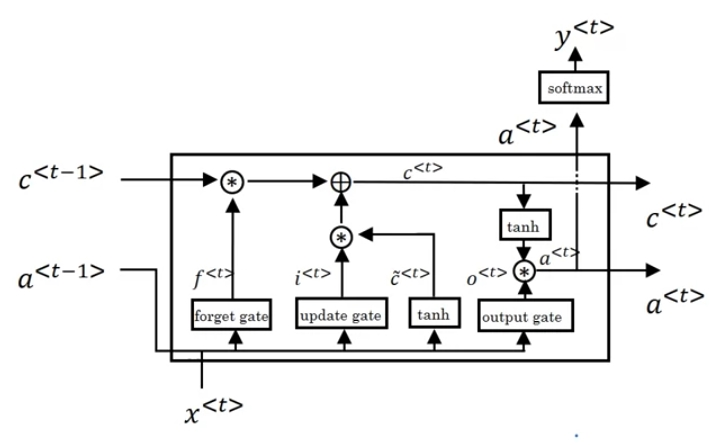
\includegraphics[scale=0.4]{Res/LSTM.jpg}
\caption{The figure to represent the LSTM.}
\label{LSTM.jpg}
\end{figure}

Historicaly, LSTM was invented first and it's more of a standard try, but GRU
are a simpler way that runs faster.

\section{Other versions of RNNs}%
\label{sec:other_versions_of_rnns}

\subsection{Bidirectional RNN}%
\label{sub:bidirectional_rnn}

BRNNs are actually very simple. We just have two RNNs, one that reads the
sequence from left to right. And other that reads the sequence from right to
left. Them, the final $\xseq[\hat{y}]{t}$ will be a combination of the outputs
of each RNN.

We denote $\overleftarrow{a}$ as the activation value of the right to left RNN,
and calculate $\xseq[\hat{y}]{t}$ as:
\[
\xseq[\hat{y}]{t}=
g\paren{W_y\sbracket{\xseq[\vec{a}]{t}, \xseq[\overleftarrow{a}]{t}}+b_y}
\]

\begin{figure}[h]
\centering
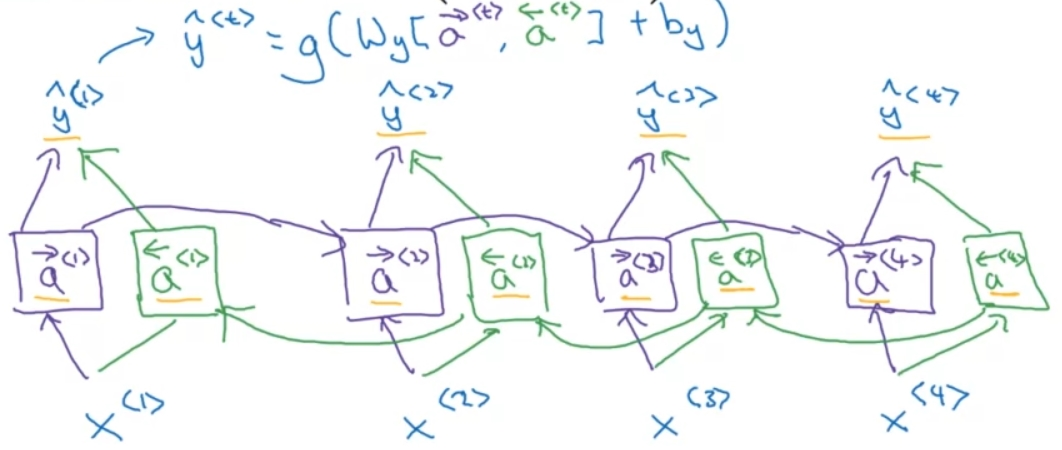
\includegraphics[scale=0.5]{Res/BRNN.jpg}
\caption{The graph of a BRNN.}
\label{BR}
\end{figure}

The disadvantage of the BRNN is that we can't predict values until we have the
whole sequence. If we have an online learning problem, we can't apply it.

\subsection{Deep RNN}%
\label{sub:deep_rnn}

Many times we need to stack RNNs together to have a deeper model that can learn
some complex function. What we've seen so far is just a single neuron that is
applied at each time to predict the output value. But indeed we can have more
than one neuron.

We'll denote $\xlayer[\xseq[a]{l}]{t}$ as the activation value for time $t$ at
layer $l$. This value is calculated using the activation from the same layer at
the previous time and the previous layer at the same time:

\[
\xlayer[\xseq[a]{l}]{t}=
g\paren{\xlayer[W_a]{l}\sbracket{
\xlayer[\xseq[a]{l}]{t-1},\xlayer[\xseq[a]{l-1}]{t}
}
+\xlayer[b_a]{l}}
\]

\begin{figure}[h]
\centering
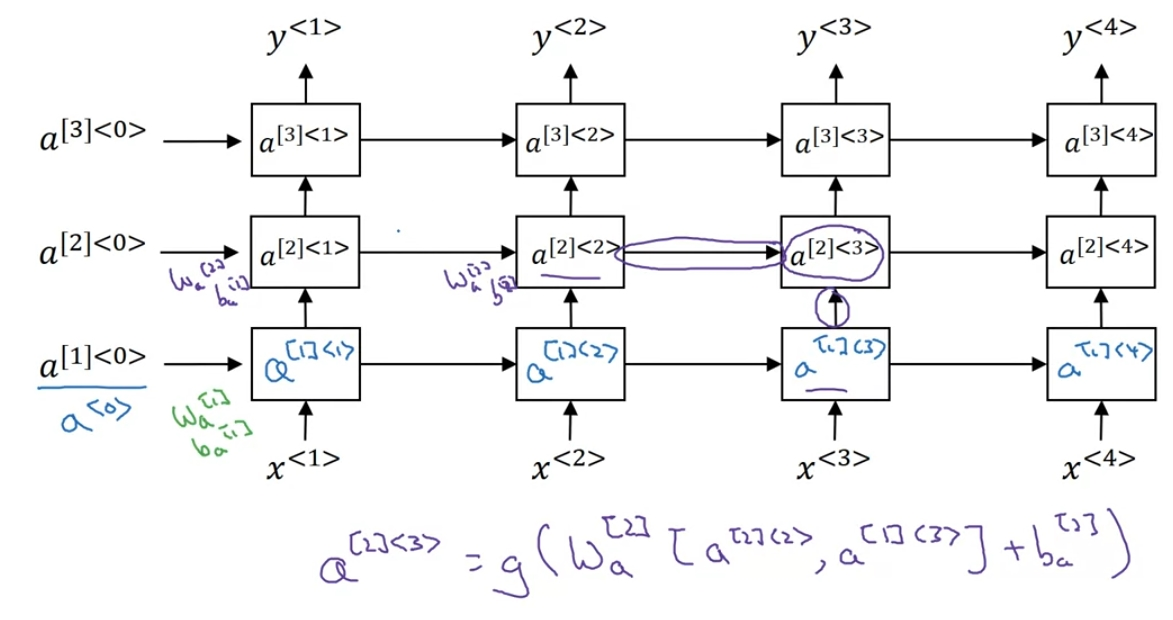
\includegraphics[scale=0.4]{Res/DRNN.jpg}
\caption{An example of Deep RNNs and how to calculate the activations.}
\label{DRNN.jpg}
\end{figure}



%%%%%%%%%%%%%%%%%%%%%%%%%%%%%%%%%%%%%%%%%%%%%%%%%%%%%%%%%%%%%%%%%%%%%%%%%%%%%%%%

\end{document}
